\documentclass[11pt]{article}
\usepackage[utf8]{inputenc}
\usepackage[T1]{fontenc}
\usepackage[margin=1.0in]{geometry}
\usepackage{amsmath,amssymb}
\usepackage{graphicx}
\usepackage{booktabs}
\usepackage{array}
\usepackage{xcolor}
\usepackage{listings}
\usepackage{caption}
\usepackage[round,authoryear]{natbib}
\usepackage{hyperref}

\definecolor{codebg}{HTML}{F6F8FA}
\definecolor{codeframe}{HTML}{D0D7DE}
\definecolor{codekw}{HTML}{0550AE}
\definecolor{codecmt}{HTML}{57606A}
\definecolor{linkblue}{HTML}{1F4E78}

\hypersetup{
    colorlinks=true,
    linkcolor=linkblue,
    citecolor=linkblue,
    urlcolor=linkblue
}

\captionsetup{font=small,labelfont=bf,skip=4pt}
\emergencystretch=1.5em

\lstset{
    basicstyle=\ttfamily\footnotesize,
    backgroundcolor=\color{codebg},
    frame=single,
    rulecolor=\color{codeframe},
    breaklines=true,
    keywordstyle=\color{codekw}\bfseries,
    commentstyle=\color{codecmt}\itshape,
    showstringspaces=false,
    tabsize=2,
    aboveskip=6pt,
    belowskip=6pt
}

% Dynamically generated statistical macros from Python pipeline
% Auto-generated by paper2_brainimation/generate_figures.py — DO NOT EDIT MANUALLY
\newcommand{\MuseBrowserKB}{37.4}
\newcommand{\LegacyMuseKB}{473.0}
\newcommand{\BundleReductionFactor}{12.6}
\newcommand{\NRefSensors}{53}
\newcommand{\NRefPFive}{38}
\newcommand{\NRefInput}{27}
\newcommand{\NRefEEGData}{19}
\newcommand{\NRefSound}{16}
\newcommand{\StudioPPGLOCMedian}{198}
\newcommand{\StudioIMULOCMedian}{215}
\newcommand{\StudioMultiLOCMedian}{120}
\newcommand{\NGamesAndEEGEdu}{43}
\newcommand{\BrainGamesLOCMedian}{514}
\newcommand{\NArchivalTotal}{121}
\newcommand{\NeurotechLOCMedian}{149}
\newcommand{\NeuroArtLOCMedian}{43}
\newcommand{\NAdditionalSketches}{26}
\newcommand{\NStarterDiag}{7}
\newcommand{\StarterDiagLOCMedian}{25}
\newcommand{\StarterDiagLOCIQRLow}{22}
\newcommand{\StarterDiagLOCIQRHigh}{120}
\newcommand{\StarterDiagLOCMin}{21}
\newcommand{\StarterDiagLOCMax}{135}
\newcommand{\NStudiosGroup}{26}
\newcommand{\StudiosLOCMedian}{200}
\newcommand{\StudiosLOCIQRLow}{130}
\newcommand{\StudiosLOCIQRHigh}{245}
\newcommand{\StudiosLOCMin}{69}
\newcommand{\StudiosLOCMax}{510}
\newcommand{\GamesEEGEduLOCMedian}{131}
\newcommand{\GamesEEGEduLOCIQRLow}{38}
\newcommand{\GamesEEGEduLOCIQRHigh}{438}
\newcommand{\GamesEEGEduLOCMin}{17}
\newcommand{\GamesEEGEduLOCMax}{758}
\newcommand{\ArchivalLOCMedian}{126}
\newcommand{\ArchivalLOCIQRLow}{50}
\newcommand{\ArchivalLOCIQRHigh}{174}
\newcommand{\ArchivalLOCMin}{12}
\newcommand{\ArchivalLOCMax}{414}
\newcommand{\StuClusterLOCMin}{87}
\newcommand{\StuClusterLOCMax}{302}
\newcommand{\WilcoxonEpochsW}{435.0}
\newcommand{\WilcoxonEpochsP}{1.86 \times 10^{-9}}
\newcommand{\EpochsExpansionFactor}{2.07}
\newcommand{\NCatalogueSketches}{234}
\newcommand{\NCatalogueCategories}{21}
\newcommand{\CatLOCMedian}{110}
\newcommand{\CatLOCIQRLow}{38}
\newcommand{\CatLOCIQRHigh}{183}
\newcommand{\CatLOCMin}{11}
\newcommand{\CatLOCMax}{1244}
\newcommand{\NPPGSketches}{10}
\newcommand{\NIMUSketches}{11}
\newcommand{\NMultiSketches}{5}
\newcommand{\NBrainGames}{14}
\newcommand{\NEEGEduModules}{13}
\newcommand{\NClassicEEGEdu}{16}
\newcommand{\NNeurotechCatalogue}{95}
\newcommand{\NNeuroArtGallery}{26}
\newcommand{\ERPNoiseRMSKOne}{17.4}
\newcommand{\ERPNoiseRMSKFive}{5.7}
\newcommand{\ERPNoiseRMSKTwenty}{2.7}
\newcommand{\ERPMCNoiseRMSKOne}{13.7}
\newcommand{\ERPMCNoiseRMSKFive}{6.1}
\newcommand{\ERPMCNoiseRMSKTwenty}{3.1}
\newcommand{\ERPSMEKOne}{8.7}
\newcommand{\ERPSMEKFive}{3.6}
\newcommand{\ERPSMEKTwenty}{1.9}
\newcommand{\ERPBlinkPtPUV}{166.2}
\newcommand{\ERPBlinkPThreeHundredBiasUV}{6.7}
\newcommand{\ERPRMSECleanTwentyUV}{3.04}
\newcommand{\ERPRMSEBlinkUnrejectedUV}{4.52}
\newcommand{\ERPRMSEBlinkRejectedUV}{3.33}
\newcommand{\JitterFCThirtyHz}{14.8}
\newcommand{\JitterFCFortyFiveHz}{9.8}
\newcommand{\JitterNullThirtyHz}{33.3}
\newcommand{\JitterNullFortyFiveHz}{22.2}
\newcommand{\JitterRetNarrowPct}{65.5}
\newcommand{\JitterRetNOneSeventyPct}{94.7}
\newcommand{\JitterRetPThreeHundredPct}{98.9}
\newcommand{\ERPSNRKOne}{0.55}
\newcommand{\ERPSNRKFive}{1.66}
\newcommand{\ERPSNRKTwenty}{3.48}
\newcommand{\EMAVarReductionPct}{98.4}
\newcommand{\FNIRSErrRawUM}{1.15}
\newcommand{\FNIRSErrCleanUM}{0.11}
\newcommand{\FNIRSErrRawUMThreeD}{1.147}
\newcommand{\FNIRSErrCleanUMThreeD}{0.113}
\newcommand{\FNIRSSuppDB}{20.1}
\newcommand{\FNIRSRRaw}{0.46}
\newcommand{\FNIRSRClean}{0.99}
\newcommand{\NLMSRMSERawUV}{43.7}
\newcommand{\NLMSRMSECleanUV}{4.8}
\newcommand{\NLMSSuppDB}{19.2}
\newcommand{\NLMSRRaw}{0.31}
\newcommand{\NLMSRClean}{0.95}
\newcommand{\NBuiltinExamples}{37}
\newcommand{\NBuiltinCategories}{10}
\newcommand{\NRefAPIs}{153}
\newcommand{\NRefGroups}{30}
\newcommand{\NRefTabs}{5}
\newcommand{\ExLOCMedian}{32}
\newcommand{\ExLOCIQRLow}{27}
\newcommand{\ExLOCIQRHigh}{38}
\newcommand{\ExLOCMin}{11}
\newcommand{\ExLOCMax}{1244}
\newcommand{\NStudentSketches}{69}
\newcommand{\NUniqueStudents}{30}
\newcommand{\StuClusterLOCMedian}{164}
\newcommand{\StuClusterLOCIQRLow}{122}
\newcommand{\StuClusterLOCIQRHigh}{173}
\newcommand{\MannWhitneyU}{2437.0}
\newcommand{\MannWhitneyClusterU}{1074.0}
\newcommand{\RankBiserialClusterR}{0.94}
\newcommand{\StuLOCMedian}{155}
\newcommand{\StuLOCMean}{157.5}
\newcommand{\StuLOCSD}{65.7}
\newcommand{\StuLOCIQRLow}{116}
\newcommand{\StuLOCIQRHigh}{189}
\newcommand{\StuLOCMin}{38}
\newcommand{\StuLOCMax}{378}
\newcommand{\NStuNF}{40}
\newcommand{\StuNFLOCMedian}{121}
\newcommand{\StuNFLOCIQRLow}{99}
\newcommand{\StuNFLOCIQRHigh}{171}
\newcommand{\StuNFLOCMin}{38}
\newcommand{\StuNFLOCMax}{378}
\newcommand{\NStuERP}{29}
\newcommand{\StuERPLOCMedian}{176}
\newcommand{\StuERPLOCIQRLow}{153}
\newcommand{\StuERPLOCIQRHigh}{221}
\newcommand{\StuERPLOCMin}{117}
\newcommand{\StuERPLOCMax}{306}
\newcommand{\StuPctCond}{66.7}
\newcommand{\StuCntCond}{46}
\newcommand{\StuPctAlpha}{53.6}
\newcommand{\StuCntAlpha}{37}
\newcommand{\StuPctRaw}{39.1}
\newcommand{\StuCntRaw}{27}
\newcommand{\StuPctBeta}{42.0}
\newcommand{\StuCntBeta}{29}
\newcommand{\StuPctERP}{42.0}
\newcommand{\StuCntERP}{29}
\newcommand{\StuPctAtt}{34.8}
\newcommand{\StuCntAtt}{24}
\newcommand{\StuPctTheta}{29.0}
\newcommand{\StuCntTheta}{20}
\newcommand{\StuPctParticles}{49.3}
\newcommand{\StuCntParticles}{34}
\newcommand{\StuPctMed}{26.1}
\newcommand{\StuCntMed}{18}
\newcommand{\StuPctAudio}{13.0}
\newcommand{\StuCntAudio}{9}
\newcommand{\StuPctEvents}{15.9}
\newcommand{\StuCntEvents}{11}
\newcommand{\NFPctCond}{57.5}
\newcommand{\NFCntCond}{23}
\newcommand{\ERPPctCond}{79.3}
\newcommand{\ERPCntCond}{23}
\newcommand{\NFPctAlpha}{92.5}
\newcommand{\NFCntAlpha}{37}
\newcommand{\ERPPctAlpha}{0.0}
\newcommand{\ERPCntAlpha}{0}
\newcommand{\NFPctBeta}{72.5}
\newcommand{\NFCntBeta}{29}
\newcommand{\ERPPctBeta}{0.0}
\newcommand{\ERPCntBeta}{0}
\newcommand{\NFPctRaw}{0.0}
\newcommand{\NFCntRaw}{0}
\newcommand{\ERPPctRaw}{93.1}
\newcommand{\ERPCntRaw}{27}
\newcommand{\NFPctAtt}{52.5}
\newcommand{\NFCntAtt}{21}
\newcommand{\ERPPctAtt}{10.3}
\newcommand{\ERPCntAtt}{3}
\newcommand{\NFPctParticles}{70.0}
\newcommand{\NFCntParticles}{28}
\newcommand{\ERPPctParticles}{20.7}
\newcommand{\ERPCntParticles}{6}
\newcommand{\CatCntAlpha}{132}
\newcommand{\CatPctAlpha}{56.4}
\newcommand{\CatCntBeta}{96}
\newcommand{\CatPctBeta}{41.0}
\newcommand{\CatCntAtt}{76}
\newcommand{\CatPctAtt}{32.5}
\newcommand{\CatCntTheta}{75}
\newcommand{\CatPctTheta}{32.1}
\newcommand{\CatCntRaw}{44}
\newcommand{\CatPctRaw}{18.8}
\newcommand{\CatCntIMU}{39}
\newcommand{\CatPctIMU}{16.7}
\newcommand{\CatCntAudio}{18}
\newcommand{\CatPctAudio}{7.7}
\newcommand{\CatCntPPG}{19}
\newcommand{\CatPctPPG}{8.1}

\raggedbottom

\title{\textbf{BrainImation: A Browser-Based Teaching Environment for Learning Creative Coding with Live EEG, Optical PPG/fNIRS, and Head Motion Sensors}}

\author{
\parbox{0.94\textwidth}{\centering
\textbf{Kyle E. Mathewson}$^{\text{a,b,*}}$, \textbf{Tamari Shalamberidze}$^{\text{b}}$, \textbf{Claire J. Scavuzzo}$^{\text{a}}$\\[5pt]
\footnotesize $^{\text{a}}$Department of Psychology, Faculty of Science, University of Alberta, Edmonton, AB, T6G 2E9, Canada\\
\footnotesize $^{\text{b}}$Neuroscience and Mental Health Institute, University of Alberta, Edmonton, AB, T6G 2E1, Canada\\
\footnotesize $^*$Correspondence: \texttt{kyle.mathewson@ualberta.ca} \ $\cdot$ \ \texttt{shalambe@ualberta.ca} \ $\cdot$ \ \texttt{scavuzzo@ualberta.ca}\\
\footnotesize Live Tool: \url{https://kylemath.github.io/Brainimation/} \ $\cdot$ \ Repository: \url{https://github.com/kylemath/Brainimation}
}
}

\date{}

\begin{document}
\maketitle

\begin{abstract}
We present BrainImation (\url{https://kylemath.github.io/Brainimation/}), a free, zero-install browser environment for behavioral neuroscience research prototyping and undergraduate laboratory instruction that connects four generations of InteraXon Muse headbands---Muse 2016, Muse~2, Classic Muse~S, and Muse~S Athena---directly to \texttt{p5.js} graphics and \texttt{p5.sound} audio in a single webpage. A self-contained WebBluetooth client (\MuseBrowserKB~KB, \BundleReductionFactor$\times$ smaller than legacy bundles) pairs with a hardware-free multi-rate signal simulator to populate a shared JavaScript object (\texttt{eegData}) providing line-filtered and raw 256~Hz EEG, Fourier band powers, 64~Hz optical pulse and forehead blood oxygenation (PPG/fNIRS), and 52~Hz 6-axis head motion, supported by a visual catalogue of \NCatalogueSketches\ sketches across \NCatalogueCategories\ categories (starting from \NStarterDiag\ one-sensor starters/diagnostics and \NBuiltinExamples\ core scaffolds, median \ExLOCMedian\ lines of code [LOC]) and a \NRefAPIs-item reference drawer. Simulation benchmarks confirm expected algorithm behavior: online ERP averaging reduces background noise across 20 trials ($\sigma_{\text{noise}}: \ERPNoiseRMSKOne \rightarrow \ERPNoiseRMSKTwenty\ \mu\text{V}$), moving-average smoothing reduces control jitter by $\EMAVarReductionPct\%$, short-channel optical regression suppresses superficial skin pulse artifacts by $\FNIRSSuppDB\text{ dB}$, and adaptive motion filtering suppresses head-movement EEG artifacts by $\NLMSSuppDB\text{ dB}$. In an upper-level cognitive neuroscience course ($N = \NStudentSketches$ exam projects from $N_{\text{students}} = \NUniqueStudents$ \texttt{PSYCH 403} students), learners expanded introductory templates into working programs (median \StuLOCMedian\ LOC; clustered $\text{median} = \StuClusterLOCMedian\text{ LOC}$, $p < 10^{-11}$), building closed-loop neurofeedback games ($N = \NStuNF$) and 4-channel ERP tasks ($N = \NStuERP$).\\[4pt]
\noindent\textbf{Keywords:} electroencephalography (EEG); functional near-infrared spectroscopy (fNIRS); photoplethysmography (PPG); brain--computer interface (BCI); event-related potential (ERP); neuroscience education
\end{abstract}

\section{Introduction}
Closed-loop brain--computer interfaces (BCIs) and neurofeedback systems turn ongoing brain, cardiac, or movement signals into real-time visual or auditory feedback so that users can observe physiological states or control interactive programs \citep{sitaram2017closed,enriquez2017eeg,lotte2013flaws}. Beyond clinical research, working with live physiological signals is a valuable hands-on way for students to learn about human neuroscience, mobile brain imaging \citep{mathewson2024moving}, media art, and brain--computer music interfacing \citep{miranda2014brain}. Over the past two decades, open-source analysis toolboxes \citep{delorme2004eeglab}, portable dry-electrode EEG headbands, and small single-board computers have made it practical to record brain activity in regular classrooms rather than shielded laboratory rooms \citep{krigolson2017choosing,mathewson2017high,kuziek2017transitioning,kuziek2018increasing}. In parallel, browser-based teaching dashboards such as \emph{EEGEdu} (\url{https://eegedu.com}) \citep{mathewson2026eegedu} allow students to inspect live brain waves, frequency spectra, and band powers in pre-built graphs. Once students understand those basic graphs, however, a common teaching question arises: how can students with little or no programming background move from passively watching pre-made charts to building their own neurofeedback games, sound synthesizers, blood-flow visualizers, and event-related potential (ERP) experiments?

\begin{figure}[t!]
\centering
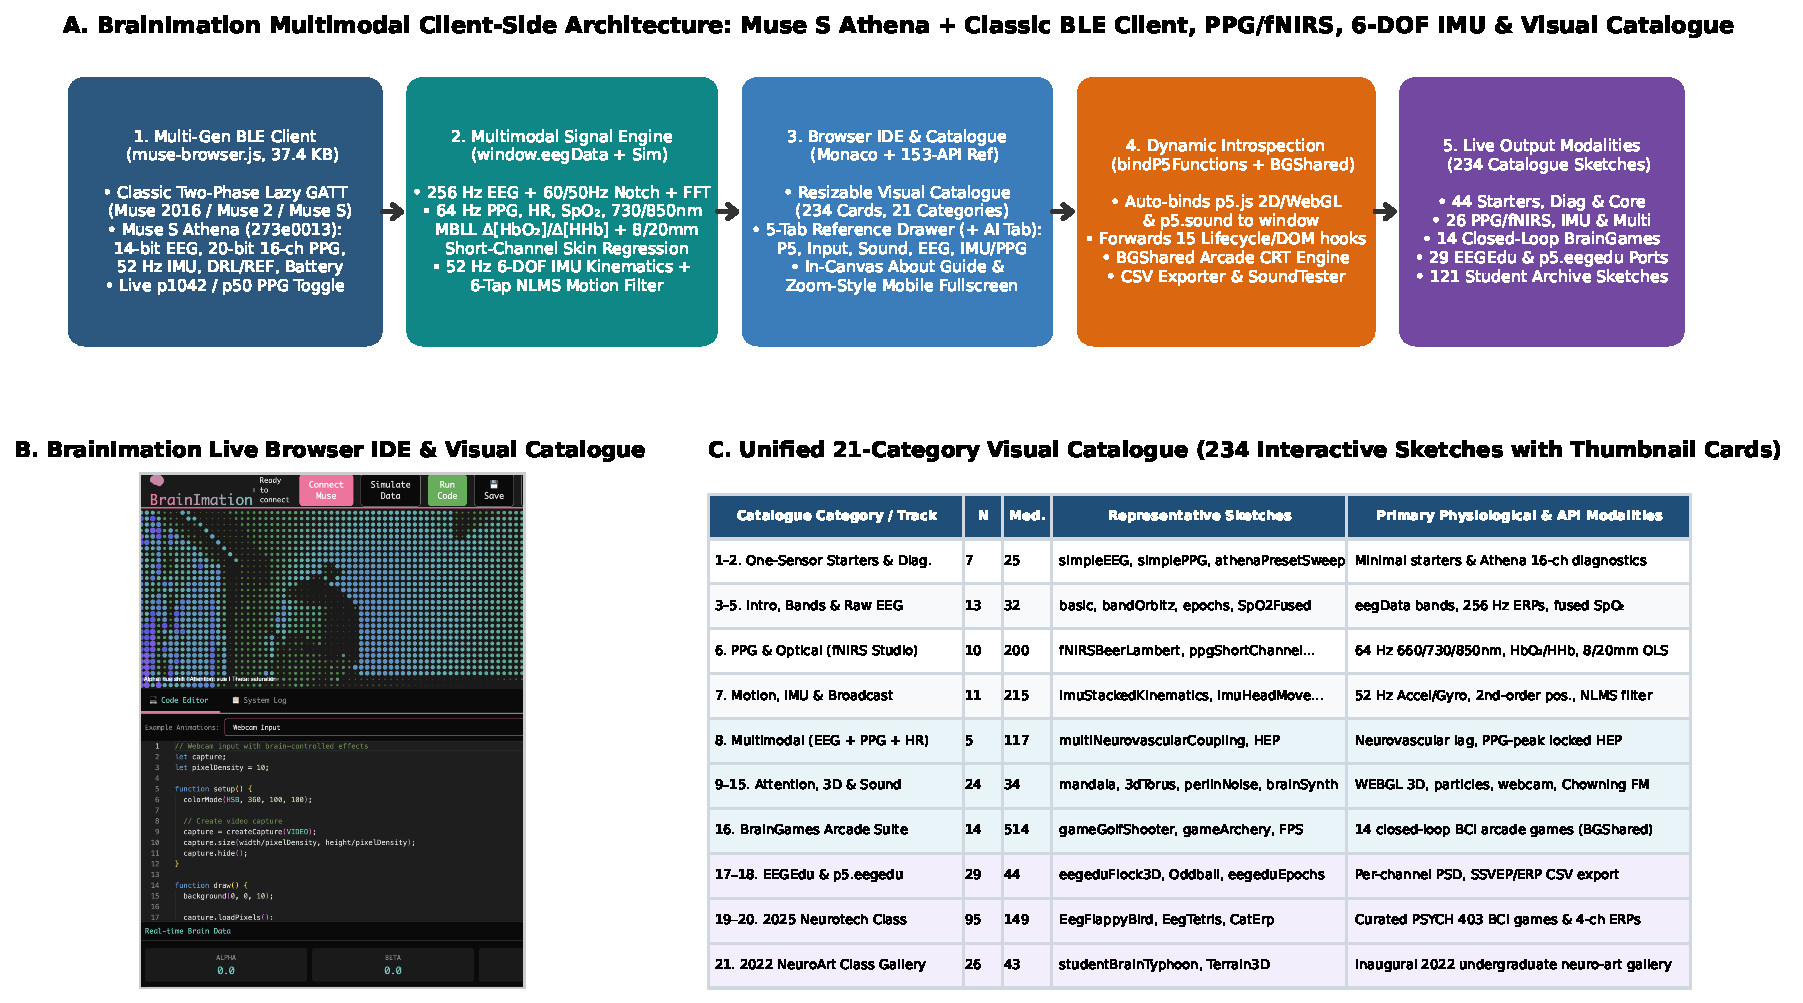
\includegraphics[width=0.98\textwidth]{figures/fig1_brainimation_ide_architecture.pdf}
\caption{\textbf{BrainImation Classroom Coding Environment and \NCatalogueCategories-Category Visual Catalogue (\NCatalogueSketches\ Sketches).} \textbf{(A)} Overview of the browser workflow: a built-in WebBluetooth connection script for Muse 2016, Muse~2, Muse~S, and Muse~S Athena headbands pairs with a hardware-free signal simulator to populate a shared \texttt{eegData} object (EEG, optical PPG/fNIRS, and 3D head motion), which drives user sketches written in the split-screen code editor with 60~FPS visual and audio output. \textbf{(B)} The BrainImation browser interface with the Visual Catalogue open. \textbf{(C)} Summary of the \NCatalogueSketches\ teaching examples and student projects organized across \NCatalogueCategories\ categories.}
\label{fig:ide}
\end{figure}

Educational programming tools such as \texttt{Processing} \citep{reas2007processing}, \texttt{Scratch} \citep{resnick2009scratch}, \texttt{p5.js} \citep{mccarthy2015p5}, and \texttt{jsPsych} \citep{deleeuw2015jspsych} follow a constructionist approach \citep{papert1980mindstorms}: beginners learn best when a tool has a ``low floor'' (making it easy to run a first working program in minutes), a ``high ceiling'' (allowing more complete experiments as skills grow), and ``wide walls'' (supporting many kinds of student projects, from visual art and music to psychology tasks). In typical BCI workflows, the starting barrier is too high for a semester course. Changing the size of a circle on screen with live alpha waves ($8\text{--}12\text{ Hz}$), forehead oxygenation, or head tilt usually requires installing an operating-system Bluetooth program, streaming data over a network socket (\texttt{LabStreamingLayer}), running a Python or C++ filtering script, and sending values to a separate graphics engine. Setting up and troubleshooting these separate programs often takes up valuable lab time before students can focus on the neuroscience concepts.

To give both researchers and students a simpler starting point for rapid neurofeedback, psychophysiology, and BCI prototyping, we created BrainImation (\url{https://github.com/kylemath/Brainimation}), a browser-based coding environment that links consumer Muse headbands---including EEG, optical pulse and blood oxygenation (PPG/fNIRS), and 3D head motion sensors---directly to the \texttt{p5.js} graphics and \texttt{p5.sound} audio libraries \citep{mccarthy2015p5} (Figure~\ref{fig:ide}). By opening a single web link in Chrome, Edge, or Opera, a researcher or student can connect a Muse headband \citep{krigolson2017choosing,kuziek2017transitioning,kuziek2018increasing}---or click \texttt{Simulate Data} in any browser when working without hardware---and run a complete neurofeedback animation in just \ExLOCMin~lines of JavaScript (\texttt{examples/basic.js}):

\noindent\begin{minipage}{\textwidth}
\begin{lstlisting}
function setup() {
  colorMode(HSB, 360, 100, 100);
}
function draw() {
  background(0, 0, 10);
  let size = map(eegData.alpha, 0, 1, 50, 300);
  let hue = map(eegData.attention, 0, 1, 180, 360);
  fill(hue, 80, 90);
  noStroke();
  ellipse(width/2, height/2, size, size);
}
\end{lstlisting}
\end{minipage}
\vspace{4pt}

In the sections that follow, we describe how BrainImation is organized for classroom use and report how undergraduate students used it in a laboratory course. Section~2 explains how the browser connects to different generations of Muse headbands and how both live and simulated signals are organized into a single \texttt{eegData} object. Section~3 describes the learning supports built into the editor, including the \NRefAPIs-item reference drawer and the visual catalogue of \NCatalogueSketches\ sketches across \NCatalogueCategories\ categories. Section~4 presents four core teaching modules---audio sonification, online ERP trial averaging, optical fNIRS superficial skin regression, and head-motion tracking with adaptive artifact filtering---showing the core code alongside simulation plots that illustrate how each method works. Finally, Section~5 reports an analysis of $N = \NStudentSketches$ examination programs written by $N_{\text{students}} = \NUniqueStudents$ undergraduate students in an upper-level cognitive neuroscience laboratory course.

\section{Connecting Headbands and Simulating Signals in the Browser}

\subsection{Supporting Four Generations of Muse Headsets (\texttt{muse-browser.js})}
In a university teaching lab, a classroom set of equipment often includes a mix of older and newer headsets bought over several years. A practical challenge for browser-based instruction is that older WebBluetooth libraries (\texttt{muse-js}) only work reliably with the original Muse 2016 headband: they fail with a connection error on Muse~2 and Classic Muse~S headbands because those headsets wait for a wake-up command before listing their sensor streams, and they do not recognize the newer Muse~S Athena headband, which packs all of its sensors into a single combined data stream. To let students connect whichever headband they are handed in lab without installing external software, BrainImation includes a lightweight (\MuseBrowserKB~KB), self-contained WebBluetooth connection script (\texttt{muse-browser.js}; Table~\ref{tab:gatt}).

\begin{table}[t!]
\centering
\caption{\textbf{Comparison of Desktop LSL Setups, Legacy Browser \texttt{muse-js}, and BrainImation's Built-In Browser Client (\texttt{muse-browser.js}).}}
\label{tab:gatt}
\footnotesize
\setlength{\tabcolsep}{5pt}
\begin{tabular}{p{0.18\textwidth}p{0.23\textwidth}p{0.23\textwidth}p{0.28\textwidth}}
\toprule
\textbf{Feature} & \textbf{Desktop LSL (\texttt{muselsl}+Py)} & \textbf{Legacy \texttt{muse-js} (v3.0)} & \textbf{BrainImation (\texttt{muse-browser.js})} \\
\midrule
Setup Required & OS BLE + Python + LSL & $\LegacyMuseKB\text{ KB}$ (\texttt{RxJS} bundle) & $\MuseBrowserKB\text{ KB}$ (No install, $\BundleReductionFactor\times$ smaller) \\
Connection Flow & Native desktop app & Single-step (fails on Muse 2/S) & Two-Step Wake-Up + Athena Decoder \\
Muse 2016 & Supported & Supported (EEG only) & Supported (EEG, IMU, Battery) \\
Muse 2 / Classic S & OS-dependent & Fails to connect & Supported (EEG, 3-Ch PPG, IMU) \\
Muse S Athena & Unsupported & Unsupported & Supported (EEG, Dual-Distance PPG/fNIRS, IMU, DRL/REF) \\
Built-In Simulator & None (Hardware req.) & Single-channel demo & 4-Ch EEG + Dual-Distance PPG/fNIRS + 3D Head Motion \\
\bottomrule
\end{tabular}
\end{table}

When a user clicks \texttt{Connect Muse}, the connection script automatically checks whether the paired headset is a Classic Muse (Muse 2016, Muse~2, or Classic Muse~S) or a Muse~S Athena. For Classic Muse headsets, the script first opens the control channel, sends a preset and stream-start command so the headset exposes its sensor streams, and then subscribes to the EEG, optical PPG, accelerometer, gyroscope, and battery streams. For the Muse~S Athena, the script subscribes to the headset's combined sensor stream and unpacks the tagged subpackets for 4- or 8-channel EEG, multi-wavelength 16-channel optical PPG/fNIRS (empirically verified using Python \texttt{bleak} hardware diagnostics in \texttt{tools/} as Red $660\text{ nm}$, Ambient, Near-Infrared $730\text{ nm}$, and Infrared $850\text{ nm}$ across short $8\text{ mm}$ and long $20\text{ mm}$ forehead spacings), 6-axis head motion, forehead contact voltages, and battery telemetry. The top toolbar also provides a \texttt{PPG: ON/OFF} button (\texttt{muse.setPPGMode(enabled)}) so users can enable forehead optical blood-flow streaming (\texttt{p1042} on Athena or \texttt{p50} on Classic) or turn the LEDs off during EEG-only exercises (\texttt{p1035}/\texttt{p21}):

\noindent\begin{minipage}{\textwidth}
\begin{lstlisting}
// Simplified two-step connection flow in muse-browser.js
// Step 1: Connect control channel first, then wake up sensor streams
this.controlChar = await this.service.getCharacteristic(CONTROL_CHAR_UUID);
await this.sendCommand('h');      // Halt previous stream
await this.sendCommand(preset);   // 'p50' (Classic EEG+PPG) or 'p1042' (Athena 16-ch optics)
await this.sendCommand('s');      // Start streaming so sensor channels appear
await this.delay(500);

// Step 2: Subscribe to Classic Muse channels or Muse S Athena combined stream (273e0013)
const chars = await this.service.getCharacteristics();
if (chars.some(c => c.uuid.includes('273e0013'))) {
  athenaChar.addEventListener('characteristicvaluechanged', e => this.parseAthenaNotification(e));
} else {
  this.bindClassicMuseStreams(chars); // EEG (256 Hz), PPG (64 Hz), IMU (52 Hz), Telemetry
}
\end{lstlisting}
\end{minipage}
\vspace{4pt}

\subsection{A Shared \texttt{eegData} Object and Built-In Simulator for Homework and Lab Use}
A central design goal for classroom use is that student code should look identical whether it is running on a physical headband in the lab or running on a student's laptop at home. To make this possible, both the live Bluetooth manager and the built-in signal simulator (\texttt{EEGSimulator}) write their outputs to the same global JavaScript object, \texttt{window.eegData}. This object organizes signals into five everyday categories that students can read inside \texttt{draw()}.

First, for frequency-band neurofeedback projects, \texttt{eegData} provides smoothed band powers scaled between $0.0$ and $1.0$ (\texttt{delta}, \texttt{theta}, \texttt{alpha}, \texttt{beta}, and \texttt{gamma}), both averaged across the headband and for each individual electrode (\texttt{TP9}, \texttt{AF7}, \texttt{AF8}, \texttt{TP10}). During live hardware recordings, 256~Hz EEG streams pass through a default-on line-noise conditioning chain (a 60~Hz or 50~Hz biquad notch filter paired with a 0.5~Hz high-pass filter, configurable via \texttt{eegData.lineFilter}), and band powers are updated from 1-second (256-sample) sliding Hanning-windowed Fourier transforms (\texttt{MuseEEGManager.calculateFrequencyBands}) after rejecting windows with large $>150\ \mu\text{V}$ eye-blink or muscle spikes, whereas the built-in signal simulator (\texttt{EEGSimulator}) drives band power envelopes directly from the interactive Attention and Meditation sidebar sliders alongside 256~Hz raw multi-channel EEG synthesis. Second, for state-monitoring and time-domain ERP tasks, \texttt{eegData} provides summary \texttt{attention} and \texttt{meditation} indices in $[0.0, 1.0]$ along with 256~Hz microvolt sample buffers (\texttt{raw}, \texttt{cleanCount}, \texttt{getRawChannel(ch, N)}, \texttt{getRecentEpoch(N)}, and \texttt{downloadCSV()}).

Third, for cardiac and optical brain-imaging lessons, \texttt{eegData} provides 64~Hz forehead photoplethysmography (PPG) and functional near-infrared spectroscopy (fNIRS) values, including the pulse waveform (\texttt{ppgPulse}), heart rate in beats per minute (\texttt{heartRate}), separate short-distance ($8\text{ mm}$) and long-distance ($20\text{ mm}$) optical channels (\texttt{ppgShort}, \texttt{ppgLong}) with optional band-pass filtering and ambient-light subtraction toggles, and real-time oxygenated and deoxygenated hemoglobin estimates ($\Delta[\text{HbO}_2]$, $\Delta[\text{HHb}]$, $\text{SpO}_2$) in \texttt{fnirsRegression}. Fourth, for movement interaction and artifact-removal lessons, \texttt{eegData} provides 52~Hz 3-axis accelerometer (\texttt{accel}) and gyroscope (\texttt{gyro}) readings, 3D head tilt angles (\texttt{orientation.pitch}, \texttt{roll}, \texttt{yaw}), 1st-order head velocity (\texttt{velocity}), 2nd-order 3D head position (\texttt{position}), and motion-cleaned EEG traces (\texttt{clean}). Fifth, for hardware diagnostics, \texttt{eegData} exposes battery level, die temperature, forehead ground voltages (\texttt{drlRef}), and per-electrode skin contact quality (\texttt{contactQuality}).

When a student clicks \texttt{Simulate Data} (Figure~\ref{fig:scaffolding}B), \texttt{EEGSimulator} generates realistic multi-channel signals across all five of these categories at their native sampling rates (256~Hz 4-channel EEG with occasional frontal eye blinks and triggered N170/P300 ERP responses, 64~Hz dual-distance optical pulse and blood-flow waves, and 52~Hz 3D head nodding and tilting) and displays Attention and Meditation sliders in the sidebar so students can test how their sketches respond to changing brain states.

\begin{figure}[t!]
\centering
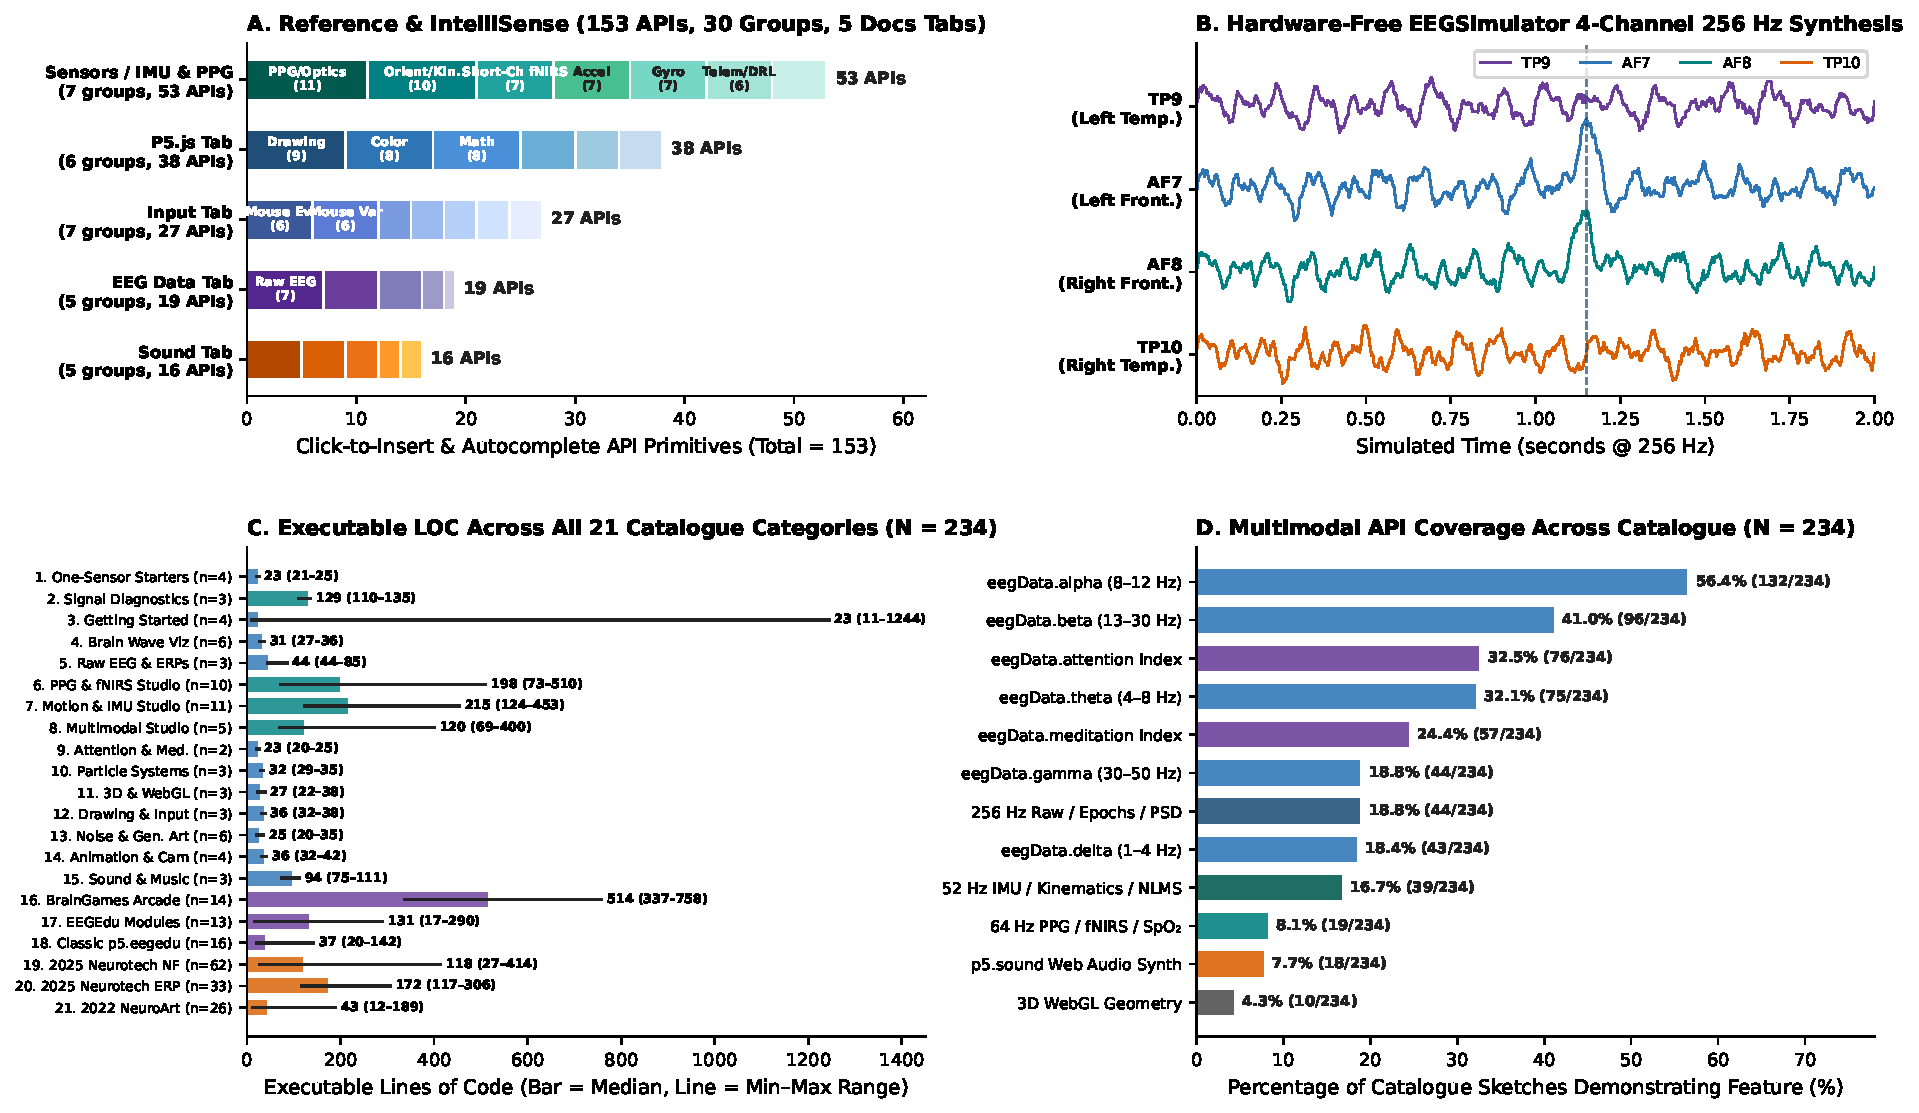
\includegraphics[width=0.98\textwidth]{figures/fig2_ide_scaffolding_and_corpus.pdf}
\caption{\textbf{Classroom Coding Supports, Hardware-Free Simulation, and \NCatalogueCategories-Category Visual Catalogue Profile ($N = \NCatalogueSketches$ Sketches).} \textbf{(A)} Distribution of the \NRefAPIs\ click-to-insert API entries across \NRefGroups\ groups and \NRefTabs\ reference tabs (\texttt{Sensors / IMU \& PPG}, \texttt{P5.js}, \texttt{Input}, \texttt{EEG Data}, and \texttt{Sound}). \textbf{(B)} Two-second 4-channel (\texttt{TP9}, \texttt{AF7}, \texttt{AF8}, \texttt{TP10}) simulated 256~Hz EEG traces from \texttt{EEGSimulator}, showing ongoing oscillations and synchronous frontal (\texttt{AF7}/\texttt{AF8}) eye blinks. \textbf{(C)} Lines of code across the \NCatalogueCategories\ categories in the Visual Catalogue ($N = \NCatalogueSketches$ sketches; bars show category median and lines span min--max range). \textbf{(D)} Percentage of the \NCatalogueSketches\ catalogue sketches demonstrating each sensor and multimedia capability.}
\label{fig:scaffolding}
\end{figure}

\section{Classroom Coding Supports and the \NCatalogueSketches-Sketch Visual Catalogue}

\subsection{Autocomplete, Click-to-Insert Reference Drawer, and Sharing Tools}
Because most psychology, neuroscience, and media-arts students enter the course with little or no JavaScript experience, the BrainImation editor includes several built-in supports to reduce typing errors and syntax frustration (Figure~\ref{fig:scaffolding}A). The left pane uses the VS Code Monaco editor configured with custom autocomplete: typing \texttt{eegData.} pops up a menu of available brain, optical, and motion properties with brief explanations. Alongside the editor, a collapsible right-hand Reference Drawer organizes \NRefAPIs\ functions and variables across \NRefTabs\ topic tabs: \emph{Sensors / IMU \& PPG} (\NRefSensors\ items), \emph{P5.js} drawing and math functions (\NRefPFive\ items), \emph{Input} mouse, keyboard, and touch handlers (\NRefInput\ items), \emph{EEG Data} properties and buffers (\NRefEEGData\ items), and \emph{Sound} synthesis tools (\NRefSound\ items), plus an optional \emph{AI Helper} tab where students can paste their own API key if permitted by the instructor. Clicking any item in the Reference Drawer shows how it works, and clicking it a second time inserts a fill-in-the-blank code snippet directly into the editor at the cursor.

To help students troubleshoot audio and share their work for grading, the top toolbar also includes a \texttt{Test Sound} button that plays a 1-second 440~Hz reference tone to wake up browser audio permissions, an \texttt{About} guide, mobile fullscreen controls, and URL sketch loading (\texttt{?sketch=}) so students and instructors can share complete playable programs via a single web link. Behind the scenes, whenever a student clicks \texttt{Run Code}, the editor automatically resets the canvas and binds all \texttt{p5.js} and \texttt{p5.sound} functions to the global window so standard introductory \texttt{p5.js} tutorials work without modification.

\subsection{The Visual Catalogue: \NCatalogueSketches\ Sketches Organized Across \NCatalogueCategories\ Categories}
Rather than asking students to start from a blank page, BrainImation includes a searchable Visual Catalogue Window (\texttt{Catalogue}) containing \NCatalogueSketches\ runnable sketches across \NCatalogueCategories\ categories ($\text{median} = \CatLOCMedian\text{ LOC}$, range $\CatLOCMin\text{--}\CatLOCMax\text{ LOC}$; Figure~\ref{fig:ide}B,C and Figure~\ref{fig:scaffolding}C,D), each shown with a preview thumbnail card. The \NCatalogueCategories\ categories are grouped into six learning tracks that progress from 11-line introductory examples to complete multimodal experiments and past student projects.

The first track begins with \NStarterDiag\ \emph{One-Sensor Starters and Signal Diagnostics} ($\text{median} = \StarterDiagLOCMedian\text{ LOC}$, range $\StarterDiagLOCMin\text{--}\StarterDiagLOCMax\text{ LOC}$, covering single-modality minimal sketches and an Athena 16-channel optical preset sweep) alongside the \emph{Core \NBuiltinCategories-Category EEG and Creative-Coding Scaffolds} ($N = \NBuiltinExamples$ sketches, $\text{median} = \ExLOCMedian\text{ LOC}$, range $\ExLOCMin\text{--}\ExLOCMax\text{ LOC}$). These short examples introduce one concept at a time across ten topics: \emph{Getting Started}, \emph{Brain Wave Visualizations}, \emph{Attention \& Meditation}, \emph{Particle Systems}, \emph{3D \& Advanced}, \emph{Drawing \& Interaction}, \emph{Raw EEG Data}, \emph{Noise \& Generative}, \emph{Animation \& Motion}, and \emph{Sound \& Music}. Students can open a 20--35 line sketch, see how a brain wave band controls color, particle speed, 3D rotation, or webcam effects, and immediately modify the numbers to test their own ideas.

Moving from brain waves to optical blood-flow sensing, the second track is the \emph{PPG and Optical (fNIRS) Studio} ($N = \NPPGSketches$ sketches, $\text{median} = \StudioPPGLOCMedian\text{ LOC}$). These visual lessons walk students step by step through forehead optical sensing: starting from a basic pulse ring and raw optical channels (ambient photodetector baseline, Red $660\text{ nm}$, Near-Infrared $730\text{ nm}$, and Infrared $850\text{ nm}$), moving to oxygenated and deoxygenated hemoglobin traces and a 6-row visual derivation of the Modified Beer--Lambert Law (pairing $660\text{ nm}/850\text{ nm}$ on Classic Muse and $730\text{ nm}/850\text{ nm}$ on Muse~S Athena, where long-path $660\text{ nm}$ photon throughput is too weak on adult foreheads), inspecting a 3D rotatable headband diagram that compares the Muse~S Athena and Muse~2 sensor layouts, comparing $8\text{ mm}$ short-channel skin signals against $20\text{ mm}$ cortical signals, and playing pulse- and breath-paced biofeedback games.

Following the same step-by-step teaching approach for movement sensors, the third track is the \emph{Motion, IMU, and Broadcast Sensors Studio} ($N = \NIMUSketches$ sketches, $\text{median} = \StudioIMULOCMedian\text{ LOC}$). Individual sketches let students explore the 3-axis accelerometer inclinometer, 3-axis gyroscope gimbal, 3D head pitch and roll horizon, battery and temperature monitors, and forehead electrode contact quality. Building on these basics, dedicated lessons visually demonstrate how raw acceleration integrates into velocity and 3D head position, how head motion can be subtracted from noisy EEG traces, and how head pitch and roll can steer musical instruments (a head-controlled theremin and beat synthesizer) or 3D tilt-labyrinth and starfield flight games.

Combining brain and cardiac signals, the fourth track is the \emph{Multimodal (EEG + PPG + HR) Studio} ($N = \NMultiSketches$ sketches, $\text{median} = \StudioMultiLOCMedian\text{ LOC}$). These examples illustrate how electrical brain activity and cardiovascular signals interact across three distinct physiological time scales: fast millisecond phase-locked ERP deflections ($50\text{--}800\text{ ms}$), sub-second to second changes in oscillatory EEG band power and beat-to-beat heart rate intervals ($0.5\text{--}2\text{ s}$), and the slower $4\text{--}6\text{ s}$ hemodynamic lag of prefrontal blood oxygenation ($\Delta[\text{HbO}_2]$ and $\Delta[\text{HHb}]$). In particular, the Heartbeat-Evoked Potential (HEP) sketch locks 256~Hz EEG epochs to the internal systolic peak of the forehead optical pulse wave rather than an external visual flash, helping students understand endogenous event-locked averaging, brain--heart interoception, and pulse transit time (PTT). Because triggering relies on the forehead PPG systolic wave rather than an ECG chest R-wave, the $\sim 150\text{--}250\text{ ms}$ baseline transit delay from ventricular depolarization and its beat-to-beat PTT jitter ($\sim 10\text{--}25\text{ ms}$) introduce physiological temporal smoothing to the recovered optical HEP relative to an ECG-gated potential.

To show how these building blocks come together in larger applications, the fifth track includes the \emph{Closed-Loop BrainGames Arcade and EEGEdu Curriculum Modules} ($N = \NGamesAndEEGEdu$ sketches total). The \emph{BrainGames} category ($N = \NBrainGames$, $\text{median} = \BrainGamesLOCMedian\text{ LOC}$) provides 14 complete neurofeedback arcade games (such as \emph{Golf Driving Range}, \emph{Archery Range}, \emph{Rowing Calm}, \emph{Balance Beam}, and \emph{Zen Breakout}) that share a common scoreboard and smoothing helper (\texttt{window.BGShared}), while \NEEGEduModules\ \emph{EEGEdu Modules} and \NClassicEEGEdu\ \emph{Classic \texttt{p5.eegedu}} sketches provide interactive versions of standard classroom labs (such as oddball ERPs and 4~Hz / 11~Hz steady-state visual evoked potentials with CSV data export).

Finally, the sixth track in the Visual Catalogue preserves two \emph{Archival Classroom Galleries} ($N = \NArchivalTotal$ student projects total): \NNeurotechCatalogue\ submissions from the \emph{2025 Neurotech Class Catalogue} ($\text{median} = \NeurotechLOCMedian\text{ LOC}$) and \NNeuroArtGallery\ projects from the \emph{2022 NeuroArt Class Gallery} ($\text{median} = \NeuroArtLOCMedian\text{ LOC}$). Keeping past student projects directly inside the catalogue gives new cohorts concrete examples of what peers with similar backgrounds were able to build. Across all \NCatalogueSketches\ catalogue sketches (Figure~\ref{fig:scaffolding}D), \texttt{eegData.alpha} is the most frequently used signal ($\CatPctAlpha\%$, $\CatCntAlpha/\NCatalogueSketches$), followed by \texttt{eegData.beta} ($\CatPctBeta\%$, $\CatCntBeta/\NCatalogueSketches$), \texttt{eegData.attention} ($\CatPctAtt\%$, $\CatCntAtt/\NCatalogueSketches$), \texttt{eegData.theta} ($\CatPctTheta\%$, $\CatCntTheta/\NCatalogueSketches$), 256~Hz raw/epoch buffers ($\CatPctRaw\%$, $\CatCntRaw/\NCatalogueSketches$), 52~Hz IMU head motion ($\CatPctIMU\%$, $\CatCntIMU/\NCatalogueSketches$), Web Audio synthesis ($\CatPctAudio\%$, $\CatCntAudio/\NCatalogueSketches$), and 64~Hz optical PPG/fNIRS ($\CatPctPPG\%$, $\CatCntPPG/\NCatalogueSketches$).

\begin{figure}[t!]
\centering
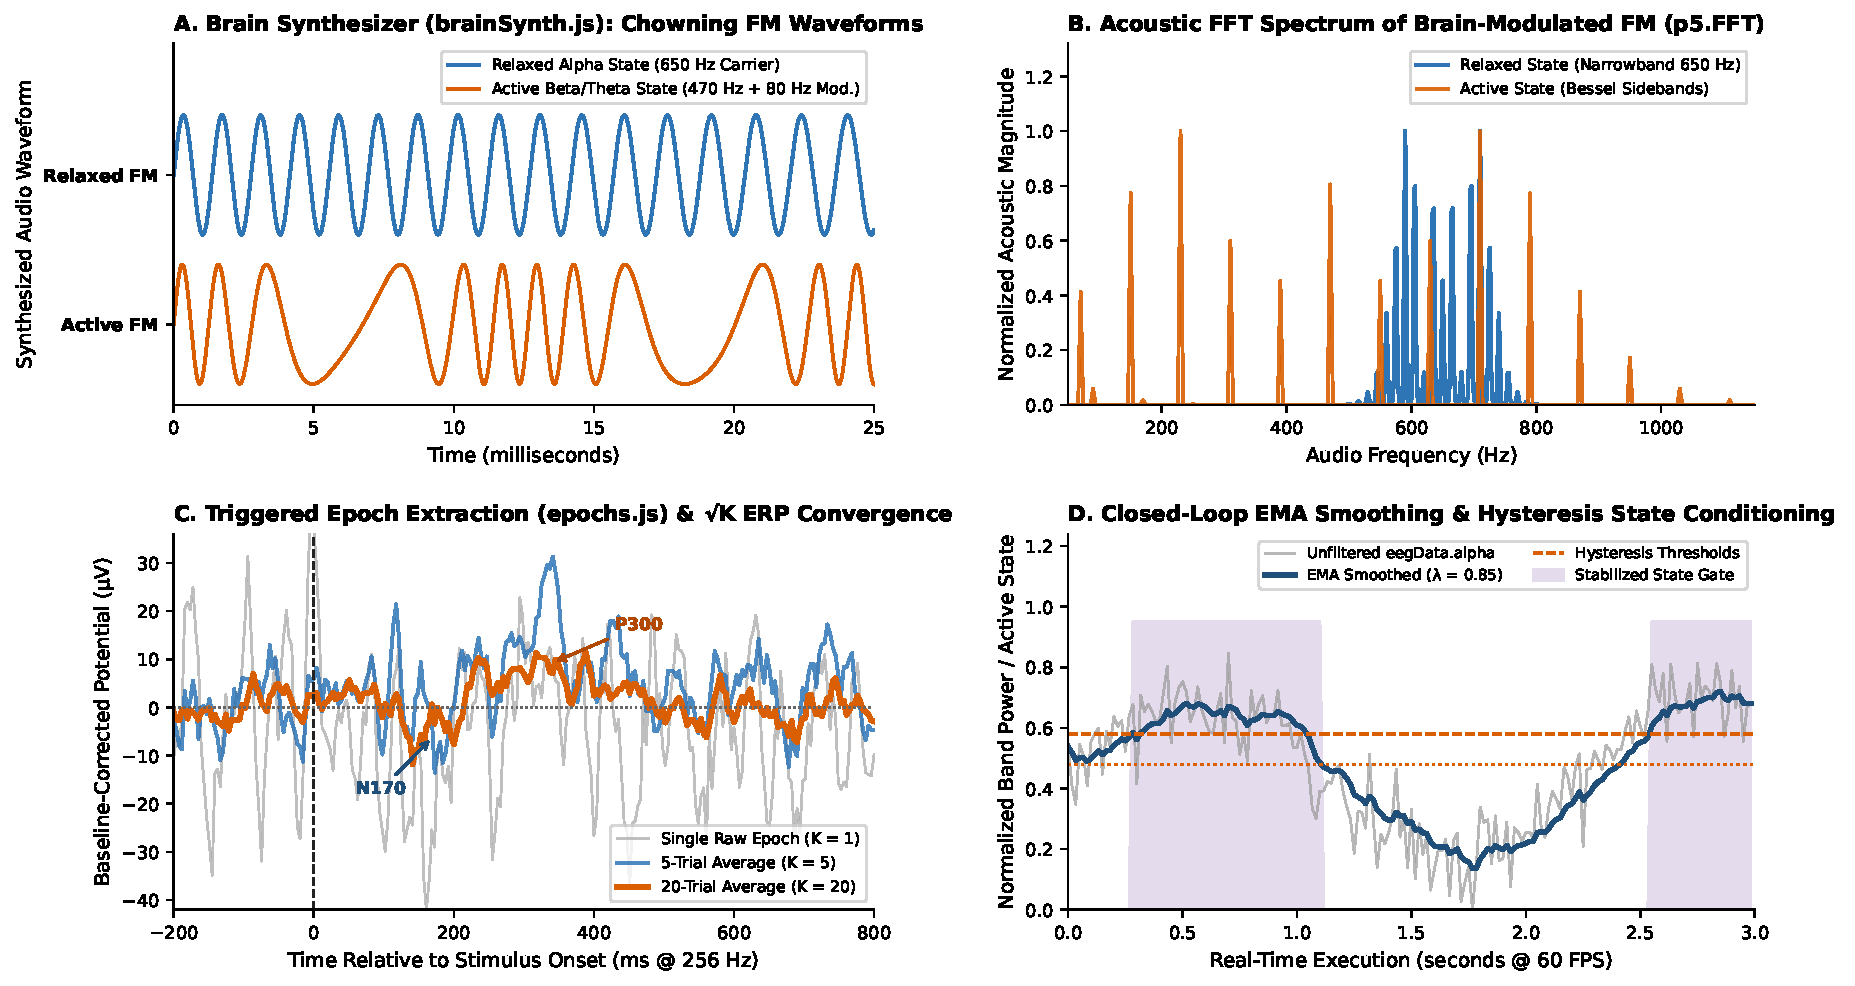
\includegraphics[width=0.98\textwidth]{figures/fig3_sonification_and_erp_engine.pdf}
\caption{\textbf{Teaching Modules for Audio Sonification, Online 4-Channel ERP Averaging, and Signal Smoothing.} \textbf{(A)} Audio waveforms from \texttt{brainSynth.js} comparing a relaxed high-alpha state ($650\text{ Hz}$ smooth tone) against an active high-beta/theta state (frequency-modulated waveform). \textbf{(B)} Corresponding audio frequency spectra (\texttt{p5.FFT}) showing a single dominant frequency during relaxation versus harmonic sidebands during active engagement. \textbf{(C)} Online 256~Hz ERP trial averaging in \texttt{epochs.js} ($-200\text{ to }+800\text{ ms}$, positive-up voltage convention in $\mu\text{V}$, baseline-corrected over $-200\text{ to }0\text{ ms}$; \citealp{picton2000guidelines,keil2014committee}) across $K = 1, 5,$ and $20$ trials. Here, \texttt{EEGSimulator} injects canonical textbook polarities ($-6.5\ \mu\text{V}$ N170 at $+170\text{ ms}$, $+9.5\ \mu\text{V}$ P300 at $+340\text{ ms}$) directly onto simulated channel \texttt{TP9} so beginners first recognize standard component morphology; by contrast, physical headband recordings measure $V_{\text{channel}} - V_{\text{Fpz}}$, which inverts vertex/parietal oddball dipoles unless re-referenced against frontal electrodes (\citealp{krigolson2017choosing}). \textbf{(D)} Exponential moving-average smoothing and dual-threshold hysteresis used in student neurofeedback games to prevent rapid on/off flicker.}
\label{fig:sonification}
\end{figure}

\section{Core Teaching Modules: Code Examples and Simulation Benchmarks}

\subsection{Audio Sonification and Frequency-Modulation Synthesis (\texttt{brainSynth.js})}
In the \emph{Sound \& Music} sketches, students learn how continuous brain wave bands can control live sound synthesis in the browser (Figure~\ref{fig:sonification}A,B). After starting with simple pitch mapping (\texttt{brainBeats.js}) and pentatonic scale notes (\texttt{alphaMusic.js}), students can open \texttt{brainSynth.js} to see how four EEG metrics control a frequency-modulation (FM) synthesizer \citep{chowning1973synthesis}. In the sketch code below, \texttt{alpha} sets the main carrier pitch, \texttt{beta} sets the modulator speed, \texttt{theta} sets the modulation depth (how rich or complex the tone sounds), and \texttt{attention} smoothly ramps the volume:

\noindent\begin{minipage}{\textwidth}
\begin{lstlisting}
// Core FM synthesis mapping from examples/brainSynth.js
let carrierFreq = map(eegData.alpha, 0, 1, 200, 800); // Alpha -> pitch (200-800 Hz)
let modFreq     = map(eegData.beta,  0, 1, 0, 100);   // Beta  -> modulation rate
let modDepth    = map(eegData.theta, 0, 1, 0, 500);   // Theta -> harmonic depth
let volume      = map(eegData.attention, 0, 1, 0, 0.2);

carrier.freq(carrierFreq);
modulator.freq(modFreq);
modulator.amp(modDepth);
carrier.amp(volume, 0.1); // 100 ms ramp prevents audio clicks between frames
\end{lstlisting}
\end{minipage}
\vspace{4pt}

As shown in the simulation plots in Figure~\ref{fig:sonification}A,B, when a user relaxes with eyes closed (high alpha, low beta and theta), the synthesizer produces a clean, steady $650\text{ Hz}$ sine wave; when beta and theta increase during active engagement, the modulator adds sideband frequencies around the carrier that students can both hear and see on the live canvas spectrum analyzer.

\subsection{Online 4-Channel ERP Averaging (\texttt{epochs.js}) and Control Smoothing}
To teach event-related potentials (ERPs), \texttt{epochs.js} shows students how time-locked averaging extracts small evoked brain responses from much larger ongoing EEG waves \citep{luck2014introduction,krigolson2017choosing} (Figure~\ref{fig:sonification}C). Because the Muse headband places its reference (\texttt{REF}) and driven right leg (\texttt{DRL}) electrodes on the center of the forehead (\texttt{Fpz}), physical posterior recordings ($V_{\text{TP9/TP10}} - V_{\text{Fpz}}$) reflect a differential potential against an active anterior site. In physical recordings, this montage reverses the polarity of classic mastoid-referenced vertex or parietal oddball dipoles unless students re-reference posterior channels against anterior electrodes ($V_{\text{TP}} - V_{\text{AF}}$; \citealp{krigolson2017choosing}) or invert the sign in software. In \texttt{EEGSimulator}, however, we intentionally inject canonical textbook polarities ($-6.5\ \mu\text{V}$ N170, $+9.5\ \mu\text{V}$ P300) directly into simulated channel \texttt{TP9} (Figure~\ref{fig:sonification}C). This ensures that beginners first recognize standard component morphology and master $\sqrt{K}$ averaging before navigating differential montage re-referencing. Every $1.5\text{ s}$ (90 frames), the sketch flashes a visual stimulus on screen. It then waits 48 frames ($+800\text{ ms}$) so the full post-stimulus response has arrived in the 256~Hz buffer, pulls the latest 256 samples ($1,000\text{ ms}$, covering $-200\text{ ms}$ before the flash to $+800\text{ ms}$ after the flash), subtracts the $-200\text{ to }0\text{ ms}$ pre-stimulus baseline average, rejects epochs with large $>100\ \mu\text{V}$ peak-to-peak eye-blink spikes, and averages the clean trial into a running grand average across all four electrodes:

\noindent\begin{minipage}{\textwidth}
\begin{lstlisting}
// Online ERP epoch extraction, blink rejection, and baseline correction (examples/epochs.js)
if (waitingForEpoch && frameCount >= stimulusFrame + 48) { // +800 ms post-stimulus
  let rawEpoch = eegData.getRecentEpoch(256); // 256 samples (1000 ms @ 256 Hz) x 4 channels
  let baselineSamples = 51;                   // First 51 samples = -200 ms to 0 ms baseline
  let hasBlink = false, baseMean = [0, 0, 0, 0];
  for (let ch = 0; ch < 4; ch++) {
    let minV = Infinity, maxV = -Infinity;
    for (let s = 0; s < 256; s++) {
      if (s < baselineSamples) baseMean[ch] += rawEpoch[s][ch] / baselineSamples;
      if (rawEpoch[s][ch] < minV) minV = rawEpoch[s][ch];
      if (rawEpoch[s][ch] > maxV) maxV = rawEpoch[s][ch];
    }
    if (maxV - minV > 100) hasBlink = true;   // >100 uV peak-to-peak whole-epoch rejection
  }
  if (!hasBlink) {                            // Update running average only on clean epochs
    trialCount++;
    for (let ch = 0; ch < 4; ch++) {
      for (let s = 0; s < 256; s++) {
        let corrected = rawEpoch[s][ch] - baseMean[ch];
        avgERP[s][ch] = ((avgERP[s][ch] * (trialCount - 1)) + corrected) / trialCount;
      }
    }
  }
  waitingForEpoch = false;
}
\end{lstlisting}
\end{minipage}
\vspace{4pt}

In theory, averaging $K$ independent trials reduces background EEG noise by a factor of $1/\sqrt{K}$ ($2.24\times$ at $K=5$ and $4.47\times$ at $K=20$), a scaling confirmed across 1,000 simulated Monte Carlo runs where the mean pre-stimulus baseline root-mean-square (RMS) noise drops from $\ERPMCNoiseRMSKOne\ \mu\text{V}$ at $K=1$ to $\ERPMCNoiseRMSKFive\ \mu\text{V}$ at $K=5$ and $\ERPMCNoiseRMSKTwenty\ \mu\text{V}$ at $K=20$. In the single illustrative realization plotted in Figure~\ref{fig:sonification}C (where random trial-to-trial fluctuations over the short 51-sample baseline window cause slight deviations from the exact $1/\sqrt{K}$ curve), the single-trial baseline RMS is $\ERPNoiseRMSKOne\ \mu\text{V}$ ($\text{SNR} = \ERPSNRKOne$), dropping to $\ERPNoiseRMSKFive\ \mu\text{V}$ at $K=5$ ($\text{SNR} = \ERPSNRKFive$) and $\ERPNoiseRMSKTwenty\ \mu\text{V}$ at $K=20$ ($\text{SNR} = \ERPSNRKTwenty$) to reveal the simulated N170 ($-6.5\ \mu\text{V}$ at $+170\text{ ms}$) and P300 ($+9.5\ \mu\text{V}$ at $+340\text{ ms}$) peaks. Correspondingly, the trial-to-trial Standardized Measurement Error ($\text{SME} = \text{SD}_{\text{trials}} / \sqrt{K}$; \citealp{luck2021standardized}) for the P300 mean amplitude window ($+280\text{ to }+400\text{ ms}$) improves from $\ERPSMEKOne\ \mu\text{V}$ ($K=1$) to $\ERPSMEKFive\ \mu\text{V}$ ($K=5$) and $\ERPSMEKTwenty\ \mu\text{V}$ ($K=20$). Including the $100\ \mu\text{V}$ peak-to-peak rejection check is equally instructive for students: when a single $115\ \mu\text{V}$ frontal eye blink ($\ERPBlinkPtPUV\ \mu\text{V}$ peak-to-peak excursion) occurs during the P300 window in 1 of the 20 trials, an unrejected average suffers up to $+\ERPBlinkPThreeHundredBiasUV\ \mu\text{V}$ of false positive bias (inflating P300-window error from $\ERPRMSECleanTwentyUV\ \mu\text{V}$ to $\ERPRMSEBlinkUnrejectedUV\ \mu\text{V}$), whereas rejecting that contaminated epoch restores the P300-window error to $\ERPRMSEBlinkRejectedUV\ \mu\text{V}$. For continuous neurofeedback games (Figure~\ref{fig:sonification}D), students also learn to smooth frame-to-frame fluctuations with a one-line exponential moving average (\texttt{smoothAlpha = 0.85 * smoothAlpha + 0.15 * eegData.alpha}), which reduces frame-to-frame jitter variance by $\EMAVarReductionPct\%$, and to use separate turn-on and turn-off thresholds (hysteresis) so game states do not flicker rapidly.

\begin{figure}[t!]
\centering
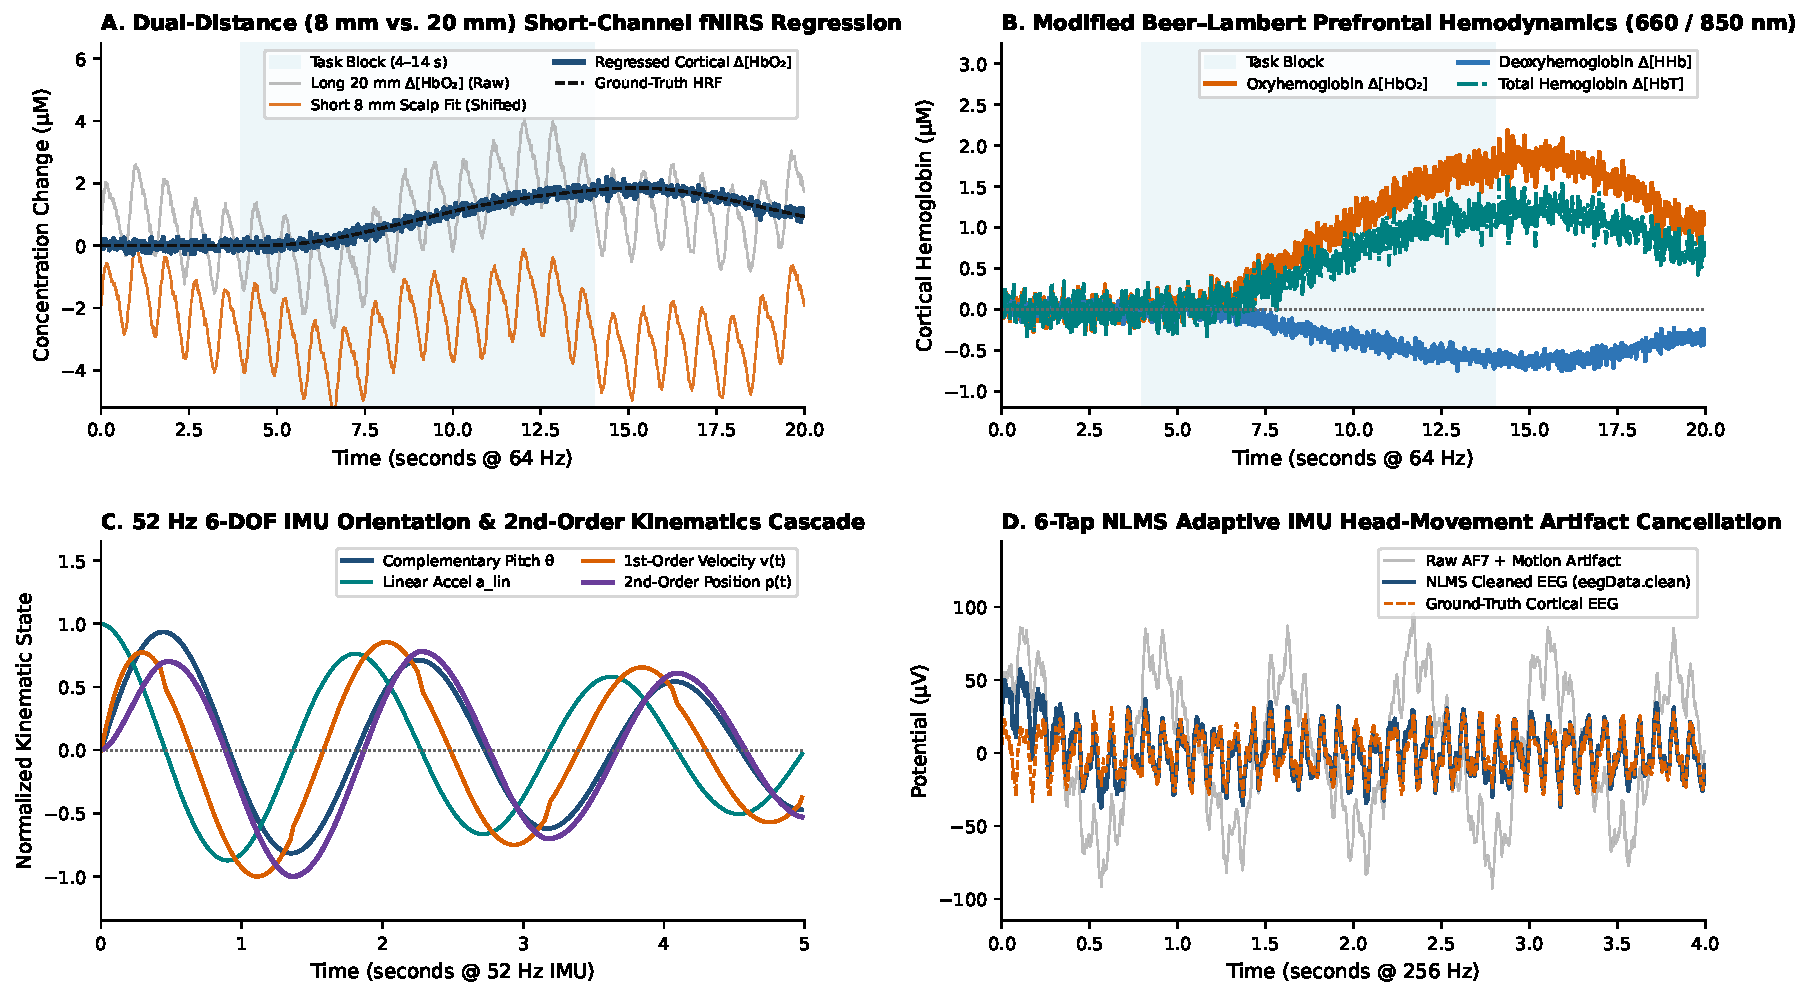
\includegraphics[width=0.98\textwidth]{figures/fig4_multimodal_athena_ppg_imu.pdf}
\caption{\textbf{Teaching Modules for Optical fNIRS Short-Channel Skin Regression and 6-DOF IMU Motion Filtering.} \textbf{(A)} Simulated dual-distance ($8\text{ mm}$ short channel vs.\ $20\text{ mm}$ long channel) optical blood-flow traces, showing how subtracting the scaled $8\text{ mm}$ superficial skin signal removes heart-pulse ($1.18\text{ Hz}$), breathing ($0.26\text{ Hz}$), and Mayer-wave ($0.10\text{ Hz}$) contamination ($\FNIRSSuppDB\text{ dB}$ reduction; $\text{RMSE}: \FNIRSErrRawUM \rightarrow \FNIRSErrCleanUM\ \mu\text{M}$ [$\FNIRSErrRawUMThreeD \rightarrow \FNIRSErrCleanUMThreeD\ \mu\text{M}$ unrounded], $r: \FNIRSRRaw \rightarrow \FNIRSRClean$). \textbf{(B)} Resulting prefrontal oxyhemoglobin ($\Delta[\text{HbO}_2]$), deoxyhemoglobin ($\Delta[\text{HHb}]$), and total hemoglobin ($\Delta[\text{HbT}]$) response during a simulated task block ($4\text{--}14\text{ s}$). \textbf{(C)} 52~Hz 6-DOF IMU head tilt angle (\texttt{pitch}, peak $\pm 16^{\circ}$), gravity-removed linear acceleration (peak $\pm 1.4\text{ m/s}^2$), 1st-order head velocity ($\text{cm/s}$), and 2nd-order 3D head displacement ($\text{cm}$), each normalized to unit peak amplitude ($[-1, 1]$) for joint comparison. \textbf{(D)} Adaptive 6-tap NLMS filtering of simulated head-movement artifacts on frontal EEG (\texttt{AF7}), reducing motion artifact by $\NLMSSuppDB\text{ dB}$ ($\text{RMSE}: \NLMSRMSERawUV \rightarrow \NLMSRMSECleanUV\ \mu\text{V}$, $r: \NLMSRRaw \rightarrow \NLMSRClean$).}
\label{fig:multimodal}
\end{figure}

\subsection{Optical PPG/fNIRS and Short-Channel Skin Regression}
The optical studio sketches introduce students to how consumer headbands measure forehead pulse and blood oxygenation using Red ($660\text{ nm}$), Near-Infrared ($730\text{ nm}$), and Infrared ($850\text{ nm}$) light \citep{delpy1988estimation,scholkmann2014review}, and how slow hemodynamic responses (peaking $4\text{--}6\text{ s}$ after cognitive task onset) differ from millisecond EEG deflections. Dual wavelengths are selected to straddle the hemoglobin isosbestic point ($\sim 800\text{ nm}$), where oxygenated ($\text{HbO}_2$) and deoxygenated ($\text{HHb}$) hemoglobin exhibit equal molar absorption: below $800\text{ nm}$ ($660\text{ nm}$ on Classic Muse; $730\text{ nm}$ on Muse~S Athena, where $660\text{ nm}$ is heavily attenuated across the $20\text{ mm}$ forehead path), $\text{HHb}$ absorption dominates, whereas at $850\text{ nm}$, $\text{HbO}_2$ dominates, providing the differential contrast required by the continuous-wave Modified Beer--Lambert Law (under the standard assumptions of constant differential pathlength factors across time and approximately homogeneous tissue scattering). In reflectance diffuse optical tomography, backscattered photons follow banana-shaped migration trajectories with an effective penetration depth of roughly $\sim d/3\text{ to }d/2$ of optode separation $d$ \citep{delpy1988estimation,saager2005direct}. Consequently, the inner $8\text{ mm}$ short channel penetrates only $\sim 2.7\text{--}4.0\text{ mm}$ (sampling exclusively superficial scalp and skull vasculature), whereas the outer $20\text{ mm}$ long channel penetrates $\sim 6.7\text{--}10.0\text{ mm}$ into superficial prefrontal cortex. Because the Muse~S Athena headband (and our simulator) provides both short and long channels, students can see how linear regression removes shallow skin hemodynamics to isolate cortical activation:

\noindent\begin{minipage}{\textwidth}
\begin{lstlisting}
// Short-channel (8 mm) vs. Long-channel (20 mm) regression in updateShortChannelRegression()
// 1. Estimate scaling factor beta between short (skin) and long (skin + brain) optical density
let covSL = 0, varS = 0;
for (let k = 0; k < W; k++) {
  let ds = shortOD[k] - meanShort;
  let dl = longOD[k]  - meanLong;
  covSL += ds * dl;
  varS  += ds * ds;
}
let beta = covSL / (varS + 1e-6);

// 2. Subtract scaled skin signal from long channel, then convert to HbO2 and HHb
let cleanOD_Red = currentLongOD_Red - betaRed * currentShortOD_Red;
let cleanOD_IR  = currentLongOD_IR  - betaIR  * currentShortOD_IR;
\end{lstlisting}
\end{minipage}
\vspace{4pt}

As shown in Figure~\ref{fig:multimodal}A,B, subtracting the scaled $8\text{ mm}$ short-channel signal from the $20\text{ mm}$ long-channel signal suppresses simulated heartbeat, breathing, and Mayer-wave skin fluctuations by $\FNIRSSuppDB\text{ dB}$, reducing the error of the recovered cortical oxyhemoglobin ($\Delta[\text{HbO}_2]$) curve from $\FNIRSErrRawUM\ \mu\text{M}$ to $\FNIRSErrCleanUM\ \mu\text{M}$ ($r = \FNIRSRRaw \rightarrow \FNIRSRClean$).

\subsection{3D Head Motion Integration and Adaptive EEG Artifact Removal}
The motion studio sketches teach two ways of using the headband's 52~Hz 3-axis accelerometer and 3-axis gyroscope. First, in the stacked kinematics lesson (Figure~\ref{fig:multimodal}C), students see how accelerometer and gyroscope readings are combined to track 3D head tilt (\texttt{pitch}, \texttt{roll}, \texttt{yaw}), how gravity is subtracted to isolate linear head acceleration, and how integrating once gives head velocity ($\text{cm/s}$) and integrating a second time gives 3D head displacement ($\text{cm}$). Second, in the adaptive motion filter lesson (Figure~\ref{fig:multimodal}D), students see how those same 6-axis motion signals can be used as a zero-lag linear spatial combiner (one instantaneous weight per IMU axis) to subtract synchronous head-movement artifacts from the EEG electrodes in real time \citep{widrow1975adaptive,mathewson2024moving}:

\noindent\begin{minipage}{\textwidth}
\begin{lstlisting}
// 6-tap adaptive (NLMS) head-movement filter in updateEEGImuMotionFilter()
let u = [0.25*linAx, 0.25*linAy, 0.25*linAz, gx/80, gy/80, gz/80]; // 6-axis IMU reference
let normU = u.reduce((sum, v) => sum + v * v, 0) + 1e-4;

for (let ch = 0; ch < 4; ch++) {
  let w = eegData.motionFilterWeights[ch];
  let estArtifact = 0;
  for (let i = 0; i < 6; i++) estArtifact += w[i] * u[i];
  let cleanEEG = eegData.raw[ch] - estArtifact; // Subtract predicted motion artifact

  // Update filter weights slightly on each sample (mu = 0.035)
  for (let i = 0; i < 6; i++) {
    w[i] = 0.9992 * w[i] + (0.035 * cleanEEG * u[i]) / normU;
  }
  eegData.clean[ch] = cleanEEG;
}
\end{lstlisting}
\end{minipage}
\vspace{4pt}

In the simulation benchmark in Figure~\ref{fig:multimodal}D, when head nodding and tilting add $\pm 85\ \mu\text{V}$ movement swings to the frontal EEG trace, the 6-tap adaptive filter learns the coupling weights within a few hundred milliseconds and reduces the synchronous motion artifact by $\NLMSSuppDB\text{ dB}$, lowering the trace error from $\NLMSRMSERawUV\ \mu\text{V}$ to $\NLMSRMSECleanUV\ \mu\text{V}$ ($r = \NLMSRRaw \rightarrow \NLMSRClean$).

\begin{figure}[t!]
\centering
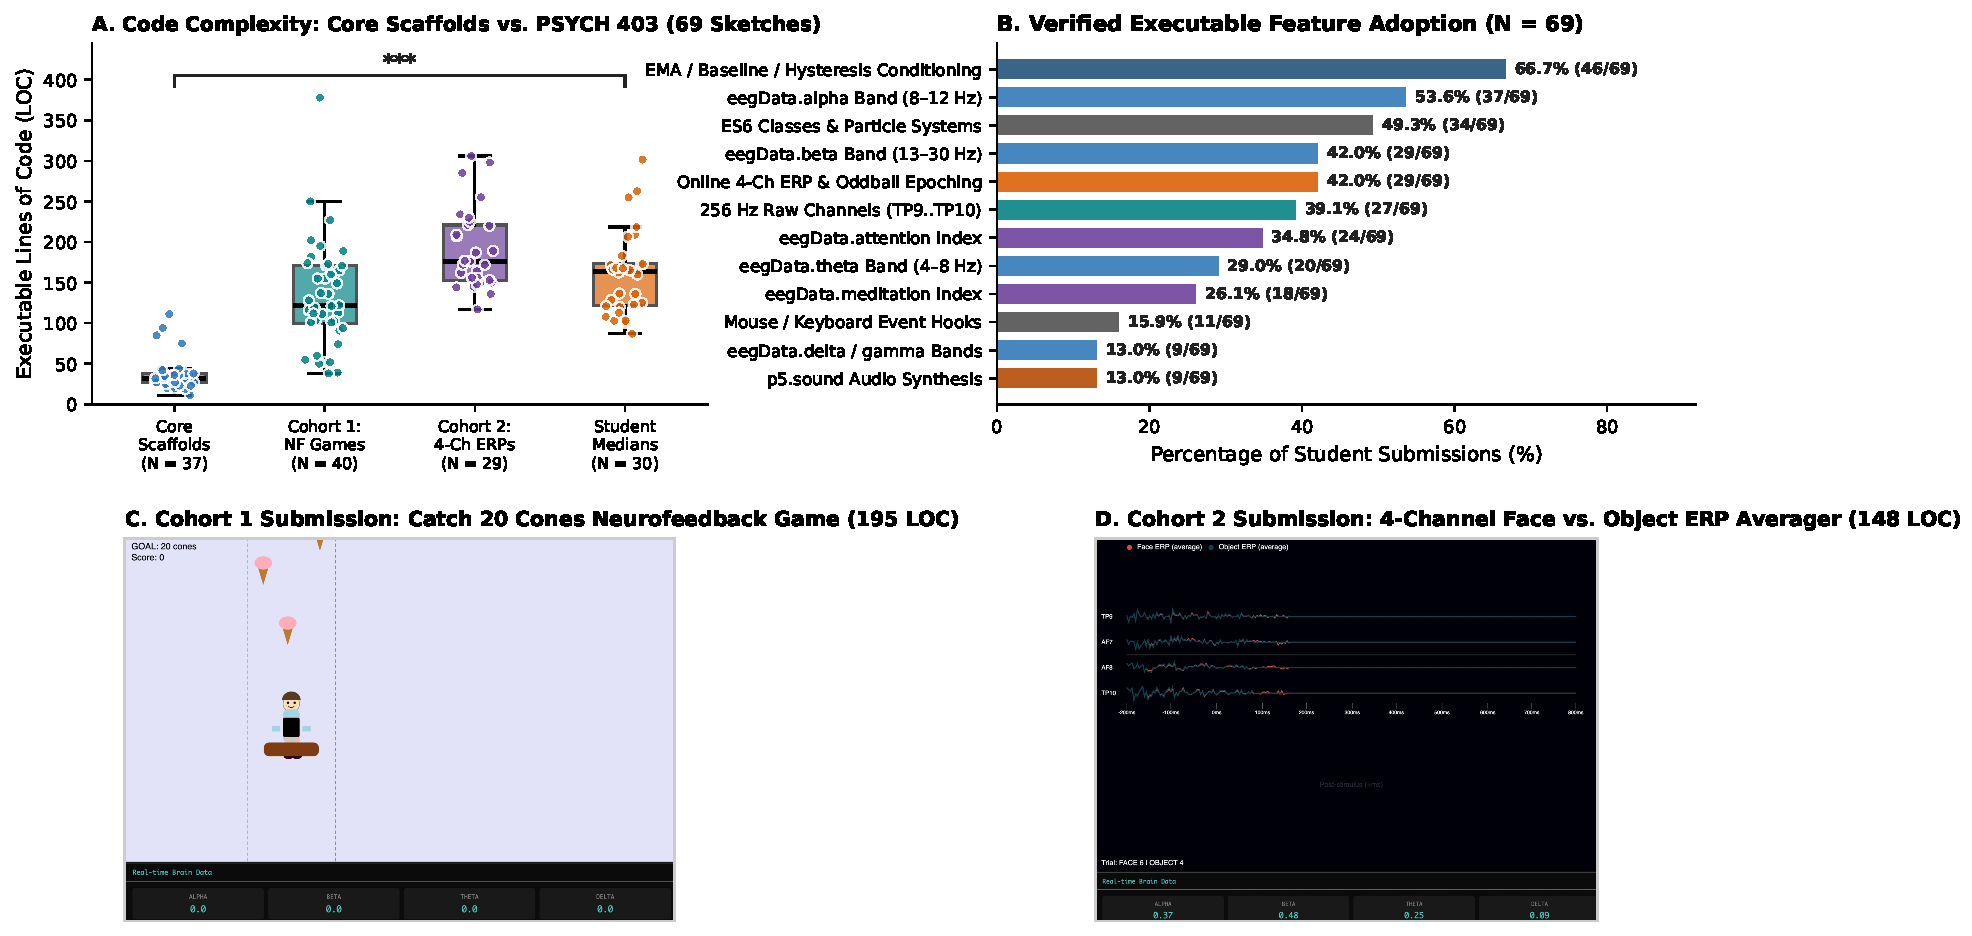
\includegraphics[width=0.98\textwidth]{figures/fig5_psych403_student_submissions_analysis.pdf}
\caption{\textbf{Classroom Evaluation of $N = \NStudentSketches$ Undergraduate Student Projects from $N_{\text{students}} = \NUniqueStudents$ Learners in \texttt{PSYCH 403}.} \textbf{(A)} Executable Lines of Code (LOC) comparing BrainImation's introductory scaffolds ($N = \NBuiltinExamples$, median $\ExLOCMedian\text{ LOC}$) against Student Cohort~1 (Neurofeedback Games \& Art; $N = \NStuNF$, median $\StuNFLOCMedian\text{ LOC}$), Student Cohort~2 (Online 4-Channel ERP Experiments; $N = \NStuERP$, median $\StuERPLOCMedian\text{ LOC}$), and per-student median lengths ($N_{\text{students}} = \NUniqueStudents$, median $\StuClusterLOCMedian\text{ LOC}$, $p < 10^{-11}$). \textbf{(B)} Percentage of student submissions using signal smoothing, EEG bands, raw ERP buffers, and interactive \texttt{p5.js} features. \textbf{(C)} Example Cohort~1 student neurofeedback game (\emph{Catch 20 Cones}, 195~LOC), showing the falling ice-cream cone sprite, horizontal catcher paddle, score/timer HUD, and bottom alpha/beta target zone indicator bar. \textbf{(D)} Example Cohort~2 student 4-channel Face vs.\ Object ERP experiment (148~LOC), showing the four color-coded electrode traces (\texttt{TP9}, \texttt{AF7}, \texttt{AF8}, \texttt{TP10}), real-time condition waveforms, and trial counter.}
\label{fig:students}
\end{figure}

\section{Classroom Evaluation (\texorpdfstring{$N = \NStudentSketches$}{N = \NStudentSketches} Projects from \texorpdfstring{$N_{\text{students}} = \NUniqueStudents$}{N\_students = \NUniqueStudents} Undergraduate Students)}

To see how undergraduate psychology and neuroscience students used BrainImation in an actual course, we examined all $N = \NStudentSketches$ verified unique examination submissions written by $N_{\text{students}} = \NUniqueStudents$ students in an upper-level cognitive neuroscience laboratory class (\texttt{PSYCH 403}, University of Alberta, Research Ethics Board Protocol \texttt{Pro00050069}; Table~\ref{tab:corpus} and Figure~\ref{fig:students}). The archive contains $N = \NStudentSketches$ submissions from $N_{\text{students}} = \NUniqueStudents$ unique learners because several students submitted iterative assignment versions (such as Assignment 2 exploratory sketches preceding Midterm Part~1, or early draft files preserved alongside revised submissions). To prevent pseudoreplication from multiple submissions per learner, we evaluated both the aggregate submission pool and a per-student clustered summary that collapses each learner's submissions into a single median value. Most students entered the class with little or no prior coding experience. Instruction followed a multi-week sequence: during guided weekly laboratory sessions, students first opened and modified the short built-in teaching scaffolds while paired with physical Muse headbands; for homework and exam preparation, they developed and debugged their own state machines on their personal laptops using \texttt{EEGSimulator} (testing threshold transitions with the Attention and Meditation sliders and verifying epoch extraction on synthetic ERP triggers); finally, they validated their finished programs on live Muse headbands in lab and submitted their code and playable \texttt{?sketch=} web links so instructors and teaching assistants could run and grade each submission directly in the browser. Each student completed two graded practical examination assignments: a continuous neurofeedback game or visualizer (Cohort~1, Midterm Part~1, $N = \NStuNF$) and an online 4-channel event-related potential experiment (Cohort~2, Midterm Part~2, $N = \NStuERP$).

\begin{table}[t!]
\centering
\caption{\textbf{Summary of Code Length and Modalities Across BrainImation's \NCatalogueSketches-Sketch Visual Catalogue and $N = \NStudentSketches$ Undergraduate Student Examination Projects ($N_{\text{students}} = \NUniqueStudents$ Students in \texttt{PSYCH 403}).} Note: The $N = \NStudentSketches$ graded examination projects (Cohort~1 $N = \NStuNF$; Cohort~2 $N = \NStuERP$) are preserved alongside \NAdditionalSketches\ additional course and laboratory sketches inside the \NNeurotechCatalogue-sketch \emph{2025 Neurotech Class Catalogue}.}
\label{tab:corpus}
\footnotesize
\setlength{\tabcolsep}{3.8pt}
\resizebox{\textwidth}{!}{%
\begin{tabular}{lcccccl}
\toprule
\textbf{Catalogue Group / Student Cohort} & \textbf{$N$} & \textbf{Med.\ LOC} & \textbf{IQR LOC} & \textbf{Min--Max} & \textbf{Primary Signals Used} & \textbf{Project Type} \\
\midrule
One-Sensor Starters \& Diagnostics & \NStarterDiag & \StarterDiagLOCMedian & $\StarterDiagLOCIQRLow\text{--}\StarterDiagLOCIQRHigh$ & $\StarterDiagLOCMin\text{--}\StarterDiagLOCMax$ & Single-sensor, 16-ch Athena & Minimal starters \& hardware checks \\
Core 10-Category Scaffolds & \NBuiltinExamples & \ExLOCMedian & $\ExLOCIQRLow\text{--}\ExLOCIQRHigh$ & $\ExLOCMin\text{--}\ExLOCMax$ & EEG bands, Att/Med, 256~Hz raw & Short introductory teaching templates \\
PPG, fNIRS, IMU \& Multimodal Studios & \NStudiosGroup & \StudiosLOCMedian & $\StudiosLOCIQRLow\text{--}\StudiosLOCIQRHigh$ & $\StudiosLOCMin\text{--}\StudiosLOCMax$ & 64~Hz PPG/fNIRS, 8/20~mm, 6-DOF IMU & Step-by-step optical \& motion lessons \\
BrainGames, EEGEdu \& Classic \texttt{p5.eegedu} & \NGamesAndEEGEdu & \GamesEEGEduLOCMedian & $\GamesEEGEduLOCIQRLow\text{--}\GamesEEGEduLOCIQRHigh$ & $\GamesEEGEduLOCMin\text{--}\GamesEEGEduLOCMax$ & Closed-loop bands, SSVEP, ERP & 14 arcade games + 29 lab modules \\
Archival Class Galleries (2022 \& 2025) & \NArchivalTotal & \ArchivalLOCMedian & $\ArchivalLOCIQRLow\text{--}\ArchivalLOCIQRHigh$ & $\ArchivalLOCMin\text{--}\ArchivalLOCMax$ & Student BCI \& NeuroArt sketches & Playable past student projects \\
\textbf{Full Visual Catalogue (\texttt{manifest.json})} & \textbf{\NCatalogueSketches} & \textbf{\CatLOCMedian} & \textbf{$\CatLOCIQRLow\text{--}\CatLOCIQRHigh$} & \textbf{$\CatLOCMin\text{--}\CatLOCMax$} & \textbf{\NCatalogueCategories\ categories with thumbnails} & \textbf{Complete in-browser sketch library} \\
\midrule
Exam Cohort 1: Neurofeedback \& Games & \NStuNF & \StuNFLOCMedian & $\StuNFLOCIQRLow\text{--}\StuNFLOCIQRHigh$ & $\StuNFLOCMin\text{--}\StuNFLOCMax$ & \texttt{eegData.alpha}, \texttt{beta}, \texttt{attention} & Student neurofeedback games \& art \\
Exam Cohort 2: Online 4-Ch ERP Tasks & \NStuERP & \StuERPLOCMedian & $\StuERPLOCIQRLow\text{--}\StuERPLOCIQRHigh$ & $\StuERPLOCMin\text{--}\StuERPLOCMax$ & 256~Hz \texttt{TP9, AF7, AF8, TP10} & Oddball P300, Face N170, Stroop, MMN \\
Per-Student Clustered Medians & \NUniqueStudents & \StuClusterLOCMedian & $\StuClusterLOCIQRLow\text{--}\StuClusterLOCIQRHigh$ & $\StuClusterLOCMin\text{--}\StuClusterLOCMax$ & One median value per student & Independent student-level summary \\
\textbf{All Exam Submissions Combined} & \textbf{\NStudentSketches} & \textbf{\StuLOCMedian} & \textbf{$\StuLOCIQRLow\text{--}\StuLOCIQRHigh$} & \textbf{$\StuLOCMin\text{--}\StuLOCMax$} & \textbf{Smoothing (\StuPctCond\%), $\alpha$ (\StuPctAlpha\%), ERP (\StuPctERP\%)} & \textbf{Graded \texttt{PSYCH 403} exam archive} \\
\bottomrule
\end{tabular}%
}
\end{table}

Here, executable LOC is defined by a simple single-clause rule: non-empty, non-comment lines of JavaScript code (excluding blank lines and lines starting with \texttt{//}, \texttt{/*}, \texttt{*}, or \texttt{*/}). Across all $N = \NStudentSketches$ examination projects, students started from the \ExLOCMedian-line introductory scaffolds and wrote working programs with a median length of \StuLOCMedian~executable lines of code ($\text{IQR} = \StuLOCIQRLow\text{--}\StuLOCIQRHigh\text{ LOC}$, range $\StuLOCMin\text{--}\StuLOCMax\text{ LOC}$; Mann--Whitney $U = \MannWhitneyU$, $p < 10^{-15}$; Figure~\ref{fig:students}A). When we grouped multiple submissions from the same person into a single median value per student ($N_{\text{students}} = \NUniqueStudents$ independent learners), the per-student median was $\StuClusterLOCMedian\text{ LOC}$ ($\text{IQR} = \StuClusterLOCIQRLow\text{--}\StuClusterLOCIQRHigh\text{ LOC}$, range $\StuClusterLOCMin\text{--}\StuClusterLOCMax\text{ LOC}$, $p < 10^{-11}$, rank-biserial correlation $r_{rb} = \RankBiserialClusterR$). In Cohort~1 ($\text{median} = \StuNFLOCMedian\text{ LOC}$), students built custom closed-loop games such as an \emph{Ice Cream Cone Catcher} driven by alpha/beta target zones (195~LOC; Figure~\ref{fig:students}C) and an \emph{EEG Flappy Bird} with adaptive difficulty (160~LOC). In Cohort~2 ($\text{median} = \StuERPLOCMedian\text{ LOC}$), students expanded the 85-line \texttt{epochs.js} scaffold into complete multi-condition ERP experiments comparing target vs.\ standard oddball stimuli or Face vs.\ Object N170 responses across all four electrodes (148~LOC; Figure~\ref{fig:students}D). Crucially, every single student submission in Cohort~2 ($29/29 = 100\%$) exceeded the 85-LOC \texttt{epochs.js} starter template (range $\StuERPLOCMin\text{--}\StuERPLOCMax\text{ LOC}$, median $\StuERPLOCMedian\text{ LOC}$, median $\EpochsExpansionFactor\times$ code expansion; Wilcoxon signed-rank $W = \WilcoxonEpochsW, p = \WilcoxonEpochsP$), demonstrating substantial student-authored experimental scaffolding.

Inspecting the non-comment lines of student code both across the combined cohort ($N = \NStudentSketches$; Figure~\ref{fig:students}B) and disaggregated by assignment type reveals how students adapted their code to each paradigm. Students implemented explicit signal conditioning---moving-average smoothing, pre-stimulus baseline subtraction, or threshold hold timers---in $\StuPctCond\%$ ($\StuCntCond/\NStudentSketches$) of all submissions, including $\NFPctCond\%$ ($\NFCntCond/\NStuNF$) of Cohort~1 neurofeedback games and $\ERPPctCond\%$ ($\ERPCntCond/\NStuERP$) of Cohort~2 ERP tasks. Continuous frequency-band and state metrics were concentrated in Cohort~1, where $\NFPctAlpha\%$ ($\NFCntAlpha/\NStuNF$; $\StuPctAlpha\%$ overall) read \texttt{eegData.alpha}, $\NFPctBeta\%$ ($\NFCntBeta/\NStuNF$; $\StuPctBeta\%$ overall) read \texttt{eegData.beta}, $\NFPctAtt\%$ ($\NFCntAtt/\NStuNF$; $\StuPctAtt\%$ overall) read \texttt{eegData.attention}, and $\NFPctParticles\%$ ($\NFCntParticles/\NStuNF$; $\StuPctParticles\%$ overall) defined custom ES6 object classes or particle systems. Conversely, time-domain buffer operations defined Cohort~2, where $100.0\%$ ($\StuCntERP/\NStuERP$; $\StuPctERP\%$ overall) implemented multi-trial ERP averaging state machines and $\ERPPctRaw\%$ ($\ERPCntRaw/\NStuERP$; $\StuPctRaw\%$ overall) indexed directly into the 256~Hz raw electrode arrays (\texttt{TP9}, \texttt{AF7}, \texttt{AF8}, \texttt{TP10}), while $\ERPPctParticles\%$ ($\ERPCntParticles/\NStuERP$) also used custom object classes to manage stimulus trials. We preserve these $N = \NStudentSketches$ graded examination files alongside \NAdditionalSketches\ additional course and laboratory sketches inside the \NNeurotechCatalogue-sketch \emph{2025 Neurotech Class Catalogue} (together with \NNeuroArtGallery\ projects from the \emph{2022 NeuroArt Class Gallery}), giving future classes a rich library of working peer examples.

\section{Discussion}
We designed BrainImation as a practical, easy-to-adopt browser environment for teaching students how to work with live physiological signals through creative coding. While companion dashboard tools such as \emph{EEGEdu} (\url{https://eegedu.com}) \citep{mathewson2026eegedu} help students understand EEG concepts through pre-built charts, BrainImation gives learners a place to write their own code using live brain waves, optical forehead blood-flow signals (PPG/fNIRS), and 3D head motion sensors \citep{papert1980mindstorms,resnick2009scratch,deleeuw2015jspsych}. By handling Bluetooth connections for Muse 2016, Muse~2, Classic Muse~S, and Muse~S Athena headsets inside the webpage, providing a built-in signal simulator for homework use, and organizing \NCatalogueSketches\ runnable examples and past student projects into a visual catalogue alongside a \NRefAPIs-item reference drawer, the tool lets classes spend their time on experimental design and signal interpretation rather than software installation.

Instructors and researchers should consider several practical limitations. First, the simulation benchmarks in Section~4 (Figures~\ref{fig:sonification} and \ref{fig:multimodal}) illustrate how the in-browser algorithms work on synthetic signals with known ground truth; they are meant as clear teaching demonstrations rather than clinical hardware validations against research-grade fNIRS or wet-electrode EEG systems. In classroom ERP labs, instructors can also have students compute the trial-to-trial Standardized Measurement Error (SME; \citealp{luck2021standardized}) in the post-stimulus component window alongside pre-stimulus baseline RMS so learners can directly compare both data-quality metrics \citep{picton2000guidelines,keil2014committee}. Second, because Bluetooth packets arrive in small bursts and browser animation loops run at $60\text{ Hz}$ ($16.67\text{ ms}$ per frame), stimulus timestamps in browser ERP tasks have $\sim 15\text{--}45\text{ ms}$ of timing jitter compared with dedicated laboratory trigger cables \citep{krigolson2017choosing,kuziek2017transitioning,kuziek2018increasing}. In the frequency domain, a uniform $30\text{ ms}$ ($45\text{ ms}$) timing jitter acts as a $\text{sinc}$ low-pass filter with a $-3\text{ dB}$ cutoff at $\JitterFCThirtyHz\text{ Hz}$ ($\JitterFCFortyFiveHz\text{ Hz}$) and a first spectral null at $\JitterNullThirtyHz\text{ Hz}$ ($\JitterNullFortyFiveHz\text{ Hz}$). Under $30\text{ ms}$ uniform jitter, a narrow $20\text{ ms}$ early sensory deflection retains only $\JitterRetNarrowPct\%$ of its peak amplitude, whereas the broader N170 ($\JitterRetNOneSeventyPct\%$ retention) and P300 ($\JitterRetPThreeHundredPct\%$ retention) components remain well preserved across 20 averaged trials and offer a useful classroom lesson on real-time timing trade-offs. Third, dry forehead and ear sensors are naturally sensitive to eye blinks, forehead muscle tension, and head movement \citep{lotte2013flaws,mathewson2017high,saager2005direct}; the built-in spike rejection, short-channel optical regression, and 6-tap adaptive IMU filter help students see how these artifacts are addressed in practice, though because the 6-tap NLMS filter uses one instantaneous weight per IMU axis, delayed mechanical settling or nonlinear electrode slip on the skin is only partially removed and does not replace careful recording habits. Fourth, pairing a physical Muse headband via WebBluetooth requires a Chromium-based browser (Chrome, Edge, Opera, or Bluefy on iOS/iPadOS), although the signal simulator and full coding editor work in Safari and Firefox on any laptop. Finally, our classroom evaluation measured the length and features of $N = \NStudentSketches$ student projects rather than pre/post exam scores, and students could draw on both the built-in examples and optional AI coding tools, so code length reflects the scope of the projects students put together rather than memorized syntax. Within these everyday classroom bounds, BrainImation provides a straightforward, zero-install way for students to learn neuroscience and physiological signal processing by building their own interactive programs.

\subsection*{Declarations}
\noindent\textbf{Open Practices Statement:} All source code (\texttt{muse-browser.js}, \texttt{index.html}, Python \texttt{bleak} hardware diagnostics in \texttt{tools/}), the live browser environment (\url{https://kylemath.github.io/Brainimation/}), all \NCatalogueSketches\ catalogue sketches and thumbnails in \texttt{examples/}, simulation benchmark generators, and the automated manuscript verification suite (\texttt{verify\_manuscript\_analyses.py}) are openly available without restriction at \url{https://github.com/kylemath/Brainimation} and \url{https://github.com/kylemath/eegeduPaper}. The classroom evaluation analyzed de-identified archival student code rather than a preregistered hypothesis test.\\[2pt]
\noindent\textbf{Ethics and SAGER Statement:} Classroom code artifacts from \texttt{PSYCH 403} were analyzed in de-identified form in accordance with procedures approved by the University of Alberta Research Ethics Board (Protocol \texttt{Pro00050069}). Because software source files were analyzed in de-identified archival form without demographic linkage, participant sex and gender dimensions were not recorded and do not affect the deterministic signal-processing benchmarks.\\[2pt]
\noindent\textbf{Data and Code Availability:} The live BrainImation environment is available at \url{https://kylemath.github.io/Brainimation/}. Source code and analysis scripts are archived at \url{https://github.com/kylemath/Brainimation} and \url{https://github.com/kylemath/eegeduPaper}.\\[2pt]
\noindent\textbf{Funding:} This work was supported by a Natural Sciences and Engineering Research Council of Canada (NSERC) Discovery Grant to K.E.M. The funding source had no involvement in study design; in the collection, analysis, and interpretation of data; in the writing of the report; or in the decision to submit the article for publication.\\[2pt]
\noindent\textbf{Declaration of Competing Interest:} The authors declare that there are no known competing financial interests or personal relationships that could have appeared to influence the work reported in this paper.\\[2pt]
\noindent\textbf{CRediT Authorship Contribution Statement:} \textbf{Kyle E. Mathewson:} Conceptualization, Methodology, Software, Validation, Formal analysis, Investigation, Resources, Data curation, Writing -- original draft, Writing -- review \& editing, Visualization, Supervision, Project administration, Funding acquisition. \textbf{Tamari Shalamberidze:} Methodology, Software, Validation, Investigation, Data curation, Writing -- review \& editing. \textbf{Claire J. Scavuzzo:} Conceptualization, Methodology, Investigation, Supervision, Writing -- review \& editing.\\[2pt]
\noindent\textbf{Declaration of Generative AI and AI-Assisted Technologies in the Manuscript Preparation Process:} During the preparation of this work the authors used large language model coding and editing assistants to verify code-to-manuscript consistency and polish prose formatting. After using these tools, the authors reviewed and edited the content as needed and take full responsibility for the content of the published article.\\[2pt]
\noindent\textbf{Acknowledgements:} The authors thank the undergraduate students and teaching assistants of \texttt{PSYCH 403} and the NeuroArt and Neurotech laboratory cohorts at the University of Alberta for testing BrainImation in the classroom.

\bibliographystyle{apalike}
\bibliography{references2}

\end{document}
